\documentclass[11pt]{article}
\usepackage[a4paper,margin=21mm]{geometry}
\usepackage[no-math]{fontspec}
\setmainfont{Latin Modern Roman}
\newfontfamily\CJKfont{Noto Serif CJK SC}
\XeTeXlinebreaklocale "zh"
\XeTeXlinebreakskip=0pt plus 1pt
\usepackage{amsmath,amssymb,amsthm,amscd,graphicx,color}
\usepackage{xurl}
\usepackage[unicode,hidelinks]{hyperref}
\allowdisplaybreaks
\setlength\emergencystretch{3em}
\numberwithin{equation}{section}

\usepackage[mathscr]{eucal} % use \EuScript (\mathcal unchanged)
%\usepackage{amsmath,amsfonts,amssymb,amsthm,amscd}
\usepackage{epic}
\usepackage{eepic}
%\usepackage{longtable}
\usepackage{array}

%\usepackage{xypic}

%\usepackage{here}
\usepackage{bm}
\usepackage[all]{xy}
\usepackage{tikz}
\usetikzlibrary{calc}

%%Tikz%%
\newcommand\qarrow[2]{\draw[->,shorten >=2pt,shorten <=2pt] (#1) -- (#2) [thick];} %arrow
\newcommand\qdarrow[2]{\draw[->,dashed,shorten >=2pt,shorten <=2pt] (#1) -- (#2) [thick];} %dashed arrow
%%

%%%%%%%%%%% Macro %%%%%%%%%%%%%%%%%
\newcommand{\Z}{{\mathbb Z}}
\newcommand{\R}{{\mathbb R}}
\newcommand{\C}{{\mathbb C}}

\newcommand{\bb}{{\mathfrak b}}
\newcommand{\e}{{\mathrm e}}

\def\ve{{\varepsilon}}
\def\vve{{\epsilon}}

\newcommand\trop{{\mathrm{trop}}}
\newcommand\rY{{\mathsf{Y}}}
\newcommand\Ad{{\mathrm{Ad}}}
\newcommand\bY{Y}
\newcommand{\qw}{{\mathcal W}}
\newcommand{\cC}{{\mathcal C}}
\newcommand{\uu}{{\mathsf u}}
\newcommand{\ww}{{\mathsf w}}

\numberwithin{equation}{section}

\newtheorem{Theorem}{Theorem}[section]
\newtheorem{Corollary}[Theorem]{Corollary}
\newtheorem{Lemma}[Theorem]{Lemma}
\newtheorem{Proposition}[Theorem]{Proposition}
 { \theoremstyle{definition}
\newtheorem{Example}[Theorem]{Example}
\newtheorem{Remark}[Theorem]{Remark} }

%% Next two commands enlarge space for figures on the top of a page
\renewcommand{\textfraction}{0.01}
\renewcommand{\topfraction}{0.99}
\makeatletter
\newcount\nativeExtraSemicolonCount
\let\nativeOriginalTikzFinish\tikz@finish
\def\nativeConsumeExtraSemicolon;{\ifnum\nativeExtraSemicolonCount=0\global\advance\nativeExtraSemicolonCount by1\else\PackageError{nativecompat}{Unexpected duplicate path delimiter}{Only the single verified source1084 duplicate delimiter is accepted}\fi}
\def\tikz@finish{\nativeOriginalTikzFinish\@ifnextchar;{\nativeConsumeExtraSemicolon}{}}
\AtEndDocument{\ifnum\nativeExtraSemicolonCount=1\typeout{NATIVE-COMPAT: exactly one verified duplicate path delimiter consumed}\else\PackageError{nativecompat}{Duplicate delimiter occurrence mismatch}{Expected exactly one consumed delimiter from source1084}\fi}
\makeatother

\makeatletter\newlabel{ss:symR}{{4.3}{}{Original source locator}{}{}}\makeatother
\begin{document}
\begin{center}\Large Parameterized tetrahedron-equation solution from a symmetric-butterfly quantum cluster quiver in the formal q-Weyl algebra for generic q\end{center}
\noindent\textbf{Stable ID:} 1053\quad\textbf{Author:} Rei Inoue; Atsuo Kuniba; Xiaoyue Sun; Yuji Terashima; Junya Yagi\par
\noindent\textbf{Work:} Solutions of Tetrahedron Equation from Quantum Cluster Algebra Associated with Symmetric Butterfly Quiver\par
\noindent\textbf{Source:} \url{https://sigma-journal.com/2024/113/}\par
\noindent\textbf{Version:} Official SIGMA 20 (2024) article 113, DOI 10.3842/SIGMA.2024.113; journal PDF and native TeX acquired 2026-09-30, exact bytes pinned by SHA256\par
\noindent\textbf{Rights:} CC BY 4.0. Authors retain copyright. \url{https://creativecommons.org/licenses/by/4.0/}. Reuse and typesetting adaptation; original language and mathematical content preserved.\par
\noindent\textbf{Difficulty (prior selection preserved):} {\CJKfont H2: The construction lifts the cluster transformations to canonical q-Weyl variables and supplies a parameter-dependent monomial operator satisfying the untwisted tetrahedron relation. A new formal-Laurent quantum-dilogarithm identity requires finiteness of each coefficient and normalization of the central scalar, after which the author conjugates the four operator blocks into the required product equality. These formal-series and operator-realization obligations remain explicit in the bundled proof.}\par
\medskip\noindent\textbf{Editorial boundary note (not author text):} Complete original main Theorem4.3 in the formal q-Weyl algebra for generic q with every canonical commutator and five-parameter constraint, explicit operator/Pijk and all current input definitions. Full cluster mutation/quantum-torus/tropical conventions and explicit symmetric-butterfly wiring/quiver data, both mutation paths, full monomial and dilogarithm arrays, complete formal coefficient-finiteness/constant-scalar argument, canonical implementation and operator-block conjugation proof are retained. The finite monomial transformations and BCH products the author terms direct/straightforward calculations remain with every input formula; no editor verification is inserted. The specific prior tropical-path equality is precisely attributed to Sun–Yagi2022 SectionA.2 as in the author proof, and formal seed synchronicity/extension facts remain exact author prerequisites. Complete AppendixA monomial information is included. Native author TikZ/xy diagrams remain editable; the one original tetra-butterfly PDF panel is unchanged with a separately marked faithful editable-label companion included with exact Figure5 panel/tier/arrow locators. One explicitly named main operator outcome; its supporting transformation/dilogarithm statements, later representations, modular double, symmetries, limits and applications are not extra counts. Literal author signs, coefficients, branch caveats and formula indices are retained without repair or new proof. Root-approved render-only TikZ path-finisher consumes exactly the one redundant second semicolon on source1084, with a compile-time occurrence assertion and errors for any other count. The literal author line, dashed arrow1-to6, all path options/labels and native source blocks remain unchanged.\par
\noindent\textbf{External original reference ss:symR:} Original symmetry-based optional normalization, source2527–2721, PDF20–22. The selected formal tetrahedron identity is proved with its explicitly defined operator and its current scalar-one dilogarithm identity; this later normalization is not an omitted proof step.\par
\medskip\hrule\medskip\noindent\textbf{Author text begins below.}\par
\setcounter{section}{1}
% Original source lines 305--2098
\section{Quantum cluster algebra}\label{s:qca}

\subsection{Mutation}\label{ss:mutation}

Let us recall the definition of quantum cluster mutation following \cite{FG06}.
For a finite set $I$, set~${B = (b_{ij})_{i,j \in I}}$ with
$b_{ij} = -b_{ji} \in \Z/2$. We call $B$ the {\it exchange matrix}.
In this article we will only encounter skew-symmetric exchange matrices
with $b_{ij} \in \bigl\{\pm 1, \pm \frac{1}{2},0\bigr\}$. An exchange matrix
will be depicted as a {\em quiver}. It is an oriented graph
with vertices labeled with the elements of $I$ and a solid arrow
(resp.\ dotted arrow) from $i$ to $j$ when $b_{ij}=1$ \big(resp.\
$b_{ij}=\frac{1}{2}$\big).

Let $\mathcal{Y}(B)$ be a skew field generated by $q$-commuting variables
$\bY = (Y_i)_{i \in I}$ under the relations
\begin{align}\label{yyq}
 Y_i Y_j = q^{2b_{ij}} Y_j Y_i.
\end{align}
The data $(B, \bY)$ will be called a quantum $y$-seed and $Y_i$ a (quantum) $Y$-variable.
We assume that the parameter $q$ is generic throughout.
%
For $(B, \bY)$ and for $k \in I$ such that
$b_{ki} \neq \pm \frac{1}{2}$, the mutation $\mu_k$ transforms
$(B, \bY)$ to $\bigl(B', \bY'\bigr) := \mu_k (B,\bY)$, where
\begin{align}\label{muB}
 &b_{ij}' =
 \begin{cases}
 -b_{ij}, & i=k \text{ or } j=k,
 \\
 \displaystyle{b_{ij} + \frac{|b_{ik}| b_{kj} + b_{ik} |b_{kj}|}{2}},
 & \text{otherwise},
 \end{cases}
 \\ \label{muY}
%
 &Y_{i}' =
 \begin{cases}
 Y_k^{-1}, & i=k,
 \\
 \displaystyle{Y_i \prod_{j=1}^{|b_{ik}|}\bigl(1 + q^{2j-1} Y_k^{-\mathrm{sgn}(b_{ik})}\bigr)^{-\mathrm{sgn}(b_{ik})}}, & i \neq k.
 \end{cases}
\end{align}
The mutations are involutive, $\mu_k \mu_k = \mathrm{id.}$, and
commutative, $\mu_k \mu_j = \mu_j \mu_k$ if $b_{jk}=b_{kj}=0$. The
mutation $\mu_k$ induces an isomorphism of skew fields
$\mu_k^{\ast}\colon \mathcal{Y}\bigl(B'\bigr) \to \mathcal{Y}(B)$, where
$\mathcal{Y}\bigl(B'\bigr)$ is a skew field generated by the variables
$Y'=\bigl(Y'_i\bigr)_{i\in I}$ under the relations
\smash{$Y'_i Y'_j = q^{2b'_{ij}} Y'_j Y'_i$}.

The map $\mu_k^{\ast}$ is decomposed into two parts, a monomial part
and an automorphism part~\cite{FG09}, in two ways \cite{Ke11}. To explain it,
let us introduce an isomorphism $\tau_{k,\varepsilon}$ of the
skew fields for~${\varepsilon \in \{+,-\}}$ by
\begin{align}\label{tauy}
\tau_{k,\ve} \colon\ \mathcal{Y}\bigl(B'\bigr) \to \mathcal{Y}(B)
; \qquad Y'_i \mapsto
\begin{cases}
 Y_k^{-1}, & i= k,
 \\
 q^{-b_{ik}[\ve b_{ik}]_+}Y_i Y_k^{[\ve b_{ik}]_+}, & i \neq k,
\end{cases}
\end{align}
where $[a]_+ := \max[0,a]$.
The adjoint action $\mathrm{Ad}_{k,\ve}$ on $\mathcal{Y}(B)$ is defined by
$\mathrm{Ad}_{k,+} := \mathrm{Ad}(\Psi_{q}(Y_k)) $, \smash{$
\mathrm{Ad}_{k,-} := \mathrm{Ad}\bigl(\Psi_{q}\bigl(Y_k^{-1}\bigr)^{-1}\bigr)$},
where $\mathrm{Ad}(Y)(X) = YXY^{-1}$.
The symbol $\Psi_q(Y)$ appearing here denotes the quantum dilogarithm
\begin{align}\label{Psiq}
\Psi_q(Y) = \frac{1}{\bigl(-qY; q^2\bigr)_\infty}, \qquad (z;q)_\infty = \prod_{n=0}^\infty (1-zq^n).
\end{align}
One has the expansions
\begin{align}\label{expa}
\Psi_q(Y) = \sum_{n = 0}^\infty \frac{(-qY)^n}{\bigl(q^2;q^2\bigr)_n},
\qquad
\Psi_q(Y)^{-1} = \sum_{n = 0}^\infty \frac{q^{n^2} Y^n}{\bigl(q^2;q^2\bigr)_n},
\end{align}
where $\bigl(z;q^2\bigr)_n = \bigl(z;q^2\bigr)_\infty/\bigl(zq^{2n};q^2\bigr)_\infty$ for any $n$.
Basic properties of the quantum dilogarithm are{\samepage
\begin{align}%\label{penta}
\label{Prec}
&\Psi_q\bigl(q^2 U\bigr) \Psi_q(U)^{-1} = 1+qU,
\\
&\Psi_q(U)\Psi_q(W) = \Psi_q(W) \Psi_q\bigl(q^{-1}UW\bigr) \Psi_q(U) \qquad \text{if}\quad UW = q^2WU,\nonumber
\end{align}
where the second one is called the pentagon identity.}

Now the decomposition of $\mu^\ast_k$ in two ways mentioned in the above
is given as
\begin{align}\label{mud}
\mu_k^{\ast} = \mathrm{Ad}_{k,+} \circ \tau_{k,+}
= \mathrm{Ad}_{k,-} \circ \tau_{k,-}.
\end{align}
Namely, one has the following diagram for both choices $\ve=+, -$:
\begin{align*}
\xymatrix{
\mathcal{Y}\bigl(B'\bigr) \ar[r]^{\mu_k^\ast} \ar[dr]_{\tau_{k,\ve}} & \mathcal{Y}(B)
\\
& \mathcal{Y}(B) \ar[u]_{\mathrm{Ad}_{k,\ve}}.
}
\end{align*}

\begin{Example}
 Let $I = \{1,2\}$ and the 2-by-2 exchange matrix be given by
 $B = \left(\begin{smallmatrix}0 & 1 \\ -1 & 0 \end{smallmatrix}\right)$, which implies
 $Y_1Y_2 = q^2Y_2Y_1$. Consider the mutation
 $\mu_2(B,\bY) = \bigl(B', \bY'\bigr)$, where $\bY = (Y_1, Y_2)$ and~${\bY' = (Y'_1, Y'_2)}$. Then $B'=-B$ from \eqref{muB} and
 \smash{$Y'_1 = Y_1\bigl(1+qY^{-1}_2\bigr)^{-1}$} from \eqref{muY}. On the other hand,
 the same result is obtained also in the form
 \smash{$Y'_1 \rightarrow Y_1\bigl(1+qY^{-1}_2\bigr)^{-1}$} in two ways according to
 \eqref{mud} as follows:
\begin{gather*}
Y'_1 \overset{\tau_{2,+}}{\longrightarrow} q^{-1}Y_1Y_2
\overset{\mathrm{Ad}_{2,+}}{\longrightarrow} q^{-1}\Psi_q(Y_2)Y_1Y_2\Psi_q(Y_2)^{-1}\\
\qquad= q^{-1}Y_1\Psi_q\bigl(q^{-2}Y_2\bigr)\Psi_q(Y_2)^{-1}Y_2
= q^{-1}Y_1\bigl(1+q^{-1}Y_2\bigr)^{-1}Y_2,
\\
Y'_1 \overset{\tau_{2,-}}{\longrightarrow} Y_1
\overset{\mathrm{Ad}_{2,-}}{\longrightarrow} \Psi_q\bigl(Y_2^{-1}\bigr)^{-1}Y_1 \Psi_q\bigl(Y_2^{-1}\bigr)
= Y_1\Psi_q\bigl(q^2Y_2^{-1}\bigr)^{-1}\Psi_q\bigl(Y_2^{-1}\bigr) =Y_1\bigl(1+qY^{-1}_2\bigr)^{-1}.
\end{gather*}
\end{Example}

For later use, we introduce the quantum torus algebra $\mathcal{T}(B)$ associated to $B$.
It is the $\mathbb{Q}(q)$-algebra generated by
non-commutative variables $\rY^\alpha$ $\bigl(\alpha \in \Z^{I}\bigr)$ satisfying the
relations
\begin{align}\label{qyy}
q^{\langle \alpha,\beta \rangle} \rY^\alpha \rY^\beta
= \rY^{\alpha + \beta},
\end{align}
where $\langle ~,~ \rangle$ is a skew-symmetric form defined by
$\langle \alpha,\beta \rangle = - \langle \beta,\alpha \rangle =
-\alpha \cdot B \beta$.
Let $e_i$ be the standard unit vector of
$\Z^I$. We write $\rY^{e_i}$ simply as $\rY_i$. Then
$\rY_i \rY_j = q^{2 b_{ij}} \rY_j \rY_i$ holds. We identify $\rY_i$ with
$Y_i$, which is consistent with \eqref{yyq}.

Let $\mathcal{FT}(B)$ be the fractional field of $\mathcal{T}(B)$.
The mutations $\mu_k^{\ast}$
and their decompositions
induce the morphisms for the fractional fields of the quantum torus algebras naturally.
%
In particular, the monomial part \eqref{tauy} of $\mu_k^{\ast}$ is written as
\begin{align}\label{taft}
\tau_{k,\ve} \colon\ \mathcal{FT}\bigl(B'\bigr) \to \mathcal{FT}(B); \qquad
\rY'_i \mapsto \begin{cases}
\rY_k^{-1}, & i= k,
\\
\rY^{e_i + e_k [\ve b_{ik}]_+}, & i \neq k
\end{cases}
\end{align}
under the identification $\rY_i = Y_i$, $\rY'_i = Y'_i$.
Hence $\mathcal{FT}(B)$ (resp. $\mathcal{FT}\bigl(B'\bigr)$) is identified with $\mathcal{Y}(B)$ (resp. $\mathcal{Y}\bigl(B'\bigr)$).

\subsection[Tropical y-variables and tropical sign]{Tropical $\boldsymbol{y}$-variables and tropical sign}

Let $\mathbb{P}(u)=\mathbb{P}_\trop(u_1,u_2,\dotsc,u_p) := \bigl\{\prod_{i=1}^{p} u_i^{a_i};\, a_i \in \Z \bigr\}$
be the tropical semifield of rank $p$, endowed with the addition $\oplus$ and multiplication $\cdot$ defined by
\[
 \prod_{i=1}^{p} u_i^{a_i} \oplus \prod_{i=1}^{p} u_i^{b_i}
 =
 \prod_{i=1}^{p} u_i^{\min(a_i,b_i)},
 \qquad
 \prod_{i=1}^{p} u_i^{a_i} \cdot \prod_{i=1}^{p} u_i^{b_i}
 =
 \prod_{i=1}^{p} u_i^{a_i+b_i}.
\]
For $s = \prod_{i \in I} u_i^{a_i} \in \mathbb{P}(u)$, we write $s = u^\alpha$
with $\alpha = (a_i)_{i \in I} \in \Z^{I}$.
We say that $s$ is positive if~${\alpha \in (\Z_{\geq 0})^{I}}$ and negative if
$\alpha \in (\Z_{\leq 0})^{I}$.

For a quiver $Q$ whose vertex set is $I$, let $\mathbb{P}(u)$ be a tropical semifield of rank $|I|$.
The data of the form $(B,y)$ with $B$ being the exchange matrix of $Q$ and
$y = (y_i)_{i \in I} \in \mathbb{P}(u)^{I}$ is called a~tropical $y$-seed.
For $k \in I$, the mutation\footnote{For simplicity, we use the same symbol $\mu_k$ to denote a mutation for
quantum $y$-seeds $(B,\bY)$ and tropical $y$-seeds $(B,y)$.}
 $\mu_k (B, y) =: \bigl(B', y'\bigr)$ is defined by
\eqref{muB} and
\begin{equation}\label{tmu}
y_{i}' =
 \begin{cases}
 y_k^{-1}, & i=k,
 \\
 y_i \bigl(1 \oplus y_k^{-\mathrm{sgn}(b_{ik})}\bigr)^{-b_{ik}}, & i \neq k.
 \end{cases}
\end{equation}
For a tropical $y$-variable $y_i' = u^{\alpha'}$, the vector $\alpha' \in \Z^I$
is called the {\it $c$-vector} of $y_i'$.
The following theorem states the {\em sign coherence} of the $c$-vectors.

\begin{Theorem}[\cite{FZ07,GHKK14}]
\label{thm:sign-coherence}
Let $\bigl(B',y'\bigr) = \mu_{i_L} \dotsm \mu_{i_2} \mu_{i_1}(B,u)$ be a
tropical $y$-seed with $y'=(y'_i)_{i \in I}$. For any sequence
$(i_1,\dotsc, i_L) \in I^L$, each $y'_i \in \mathbb{P}(u)$ is either
positive or negative.
\end{Theorem}

Based on Theorem \ref{thm:sign-coherence}, for any tropical $y$-seed $\bigl(B',y'\bigr)$ with
$y'=(y'_i)_{i \in I}$ obtained from $(B,u)$ by applying mutations, we
define the {\it tropical sign} $\ve_i'$ of $y_i'$ to be $+1$ (resp.\
$-1$) if $y_i'$ is positive (resp.\ $y_i$ is negative). We also write
$\ve_i'= \pm$ for $\ve_i'=\pm 1$ for simplicity.

\begin{Remark}\label{re:sgni}
For the mutation $\mu_k (B,y) = \bigl(B',y'\bigr)$ of a tropical $y$-seed,
let $c_i$, $c_i'$, $c_k$ be the $c$-vectors of $y_i$, $y_i'$, $y_k$, respectively,
and let $\ve_k$ be the tropical sign of $y_k$.
Then the tropical mutation \eqref{tmu} is expressed in terms of $c$-vectors as
\begin{align*}
 c_i' =
 \begin{cases}
 -c_k, & i=k,
 \\
 c_i + c_k [\ve_k b_{ik}]_+, & i \neq k.
\end{cases}
\end{align*}
This coincides with the transformation of quantum torus \eqref{taft}
on $\Z^I$ (i.e., the power of \eqref{taft}) when $\ve = \ve_k$.
\end{Remark}

\subsection{Sequence of mutations}

Let us describe the quantum $Y$-variables associated with the sequence
of mutations $\mu_{i_l} \mu_{i_{l-1}} \dots \allowbreak\mu_{i_2} \mu_{i_1}$:
 \begin{align}\label{bys}
\bigl(B^{(1)},\bY^{(1)}\bigr) \stackrel{\mu_{i_1}}{\longleftrightarrow}
\bigl(B^{(2)},\bY^{(2)}\bigr) \stackrel{\mu_{i_2}}{\longleftrightarrow}
\cdots
\stackrel{\mu_{i_l}}{\longleftrightarrow} \bigl(B^{(l+1)},\bY^{(l+1)}\bigr).
\end{align}
%
For $t=1, \dots, l+1$, let $\rY^\alpha(t)$ $\bigl(\alpha \in \Z^I\bigr)$ be the
generators of the quantum torus $\mathcal{T}\bigl(B^{(t)}\bigr)$ in the sense
explained around \eqref{qyy}. We set $\rY_i(t) =
\rY^{e_i}(t)$.
Especially for $t=1$, we use the simpler notations
$\rY^\alpha=\rY^\alpha(1)$ and $\rY_i=\rY_i(1)$. As in \eqref{taft},
we identify $\rY_i$ with \smash{$Y_i = Y^{(1)}_i$}, hence
\smash{$\mathcal{Y}\bigl(B^{(1)}\bigr)$} with \smash{$\mathcal{FT}\bigl(B^{(1)}\bigr)$}.
%
Then the quantum $Y$-variables \smash{$Y^{(t+1)}=\bigl(Y^{(t+1)}_i\bigr)_{i\in I}$}
($t=0, \dots, l$) appearing in~\eqref{bys} are expressed as
\begin{align}
Y_i^{(t+1)}
&= \Ad\bigl(\Psi_{q}\bigl(\rY_{i_1}(1)^{\delta_1}\bigr)^{\delta_1}\bigr) \tau_{i_1,\delta_1}\dotsm \Ad\bigl(\Psi_{q}\bigl(\rY_{i_{t}}(t)^{\delta_{t}}\bigr)^{\delta_{t}}\bigr) \tau_{i_{t},\delta_{t}}(\rY_i(t+1))\nonumber
\\
&=\Ad\bigl(\Psi_{q}\bigl(\rY^{\delta_1 \beta_1}\bigr)^{\delta_1} \dotsm \Psi_{q}\bigl(\rY^{\delta_{t} \beta_{t}}\bigr)^{\delta_{t}}\bigr) \tau_{i_1,\delta_1}\dotsm \tau_{i_{t},\delta_{t}}(\rY_i(t+1)).\label{yad}
\end{align}
This formula is valid for any choice of the signs $\delta_1, \dots,
\delta_l \in \{+, -\}$, on which the left-hand side is independent. Note that
\smash{$Y^{(t+1)}_i$} is in general a ``complicated'' element in
$\mathcal{Y}\bigl(B^{(1)}\bigr)$ generated from \smash{$\bigl(B^{(1)},Y^{(1)}\bigr)$} by applying
$\mu_{i_t}\dotsm \mu_{i_2}\mu_{i_1}$ according to \eqref{muY}.
On the other hand,
$\rY_i(t+1)$ is just a basis of \smash{$\mathcal{T}\bigl(B^{(t+1)}\bigr)$}. The first
line of \eqref{yad} says that \smash{$Y^{(t+1)}_i$} is also obtained as the
image of $\rY_i(t+1)$ under the composition
\smash{$\mu_{i_1}^\ast \dotsm \mu^\ast_{i_{t-1}} \mu^\ast_{i_t}$} which is an
isomorphism
$\mathcal{FT}\bigl(B^{(t+1)}\bigr) \rightarrow \mathcal{FT}\bigl(B^{(1)}\bigr) =
\mathcal{Y}\bigl(B^{(1)}\bigr)$. The second line is derived from the first line
by pushing $\tau_{i,\delta}$'s to the right. Thus we have $\beta_1 = e_{i_1}$,
and in general $\beta_r \in \Z^I$ is determined by
$\rY^{\beta_r} = \tau_{i_1,\delta_1} \dotsm \tau_{i_{r-1},
 \delta_{r-1}}(\rY_{i_r}(r))$.


\subsection{A useful theorem}

Let $\sigma_{r,s} \in \mathfrak{S}_I$ ($r, s \in I$) be a transposition.
We let it act on either classical $y$-seeds $(B,y)$ or quantum $y$-seeds $(B,Y)$
as the exchange of the indices $r$ and $s$. For quantum $y$-seeds, it
is given~by
\begin{equation}\label{qys}
((b_{ij})_{i,j\in I} , (Y_i)_{i \in I} ) \mapsto
((b_{\sigma_{r,s}(i), \sigma_{r,s}(j)})_{i,j\in I}, (Y_{\sigma_{r,s}(i)})_{i \in I} ),
\end{equation}
where $\sigma_{r,s}(r) = s$, $\sigma_{r,s}(s)=r$ and
$\sigma_{r,s}(i) = i$ for $i \neq r,s$. For classical $y$-seeds, the
rule is similar.

Let
\begin{equation}\label{nuL}
\nu = \nu_L\dotsm \nu_1 := \sigma_{r_m,s_m} \dotsm
\mu_{i_l} \dotsm \sigma_{r_1,s_1} \dotsm \mu_{i_1}, \qquad L = l+m,
\end{equation}
be a composition of $l$ mutations $\mu_{i_1}, \dots, \mu_{i_l}$ and
$m$ transpositions $\sigma_{r_1,s_1}, \dots, \sigma_{r_m, s_m}$ in
an arbitrary order. (So $\nu_L$ may actually be a mutation for
example.) For simplicity, we also call $\nu$ a~mutation sequence even
though a part of it may involve transpositions.

Consider the tropical $y$-seeds starting from $(B,y)$ and the quantum
$y$-seeds starting from $(B,Y)$ which are generated along the mutation
sequences $\nu=\nu_L\dotsm \nu_1$ and $\nu'= \nu'_{L'} \dotsm \nu'_1$
as follows:
\begin{align}%\label{seq1}\label{seq2}
\label{seq0}
&(B,y) =:\bigl(B^{(1)},y^{(1)}\bigr) \stackrel{\nu_1}{\longleftrightarrow}
\bigl(B^{(2)},y^{(2)}\bigr) \stackrel{\nu_2}{\longleftrightarrow}
\dotsb
\stackrel{\nu_L}{\longleftrightarrow} \bigl(B^{(L+1)},y^{(L+1)}\bigr) = \nu(B,y),
\\
&(B,\bY) =:\bigl(B^{(1)},\bY^{(1)}\bigr) \stackrel{\nu_1}{\longleftrightarrow}
\bigl(B^{(2)},\bY^{(2)}\bigr) \stackrel{\nu_2}{\longleftrightarrow}
\dotsb
\stackrel{\nu_L}{\longleftrightarrow} \bigl(B^{(L+1)},\bY^{(L+1)}\bigr) = \nu(B,Y),
\\
&(B,y) =:\bigl(B^{(1)\prime },y^{(1)\prime}\bigr) \stackrel{\nu'_1}{\longleftrightarrow}
\bigl(B^{(2)\prime},y^{(2)\prime}\bigr) \stackrel{\nu'_2}{\longleftrightarrow}
\dotsb
\stackrel{\nu'_{L'}}{\longleftrightarrow} \bigl(B^{(L+1)\prime},y^{(L+1)\prime}\bigr) = \nu'(B,y),
\\
&(B,\bY) =:\bigl(B^{(1)\prime},\bY^{(1)\prime}\bigr) \!\stackrel{\nu'_1}{\longleftrightarrow}\!
\bigl(B^{(2)\prime},\bY^{(2)\prime}\bigr) \!\stackrel{\nu'_2}{\longleftrightarrow}
\dotsb
\stackrel{\nu'_{L'}}{\longleftrightarrow} \!\bigl(B^{(L+1)\prime},\bY^{(L+1)\prime}\bigr) = \nu'(B,Y).\!\!\!
\label{seq3}
\end{align}
The following theorem is established by combining the synchronicity \cite{N21}
among $x$-seeds, $y$-seeds and tropical $y$-seeds,
and the synchronicity between classical and quantum seeds
\cite[Lemma 2.22]{FG09b}, \cite[Proposition~3.4]{KN11}.

\begin{Theorem}\label{thm:piv}
 In the situation in \eqref{seq0}--\eqref{seq3}, the following two
 statements are equivalent:
\begin{itemize}\itemsep=0pt

\item[$(1)$]
The tropical $y$-seeds satisfy $\nu (B,y) = \nu'(B,y)$.

\item[$(2)$]
The quantum $y$-seeds satisfy $\nu (B,\bY) = \nu'(B,\bY)$.

\end{itemize}
\end{Theorem}

It is remarkable that (2) follows from (1) which is much simpler to check.
We will utilize this fact efficiently
in the subsequent arguments.


\section[Cluster transformation R]{Cluster transformation $\boldsymbol{\widehat{R}}$}\label{s:ct}

\subsection{Wiring diagram and symmetric butterfly quiver}

Let us fix our convention of the wiring diagrams and associated square quivers
using examples.
See also \cite[Section 3]{SY22}.
%
Let $W(A_n)$ be the Weyl group of $A_n$ generated by the simple
reflections~${s_1,\dotsc, s_n}$ obeying the Coxeter relations $s_i^2=1$,
$s_is_js_i = s_js_is_j$ ($|i-j|=1$) and~${s_is_j=s_js_i}$~($|i-j|\ge 2$). A reduced expression
$s_{i_1}\dotsm s_{i_l}$ of an element in $W(A_n)$ is identified with
the (reduced) word $i_1\ldots i_l \in [1,n]^l$. A wiring diagram is a
collection of $n$ wires which are horizontal except the vicinity of
crossings. In the aforementioned context, $i_k$ indicates that the
$k$-th crossing from the left takes place at the $i_k$-th level,
measured from the top. Crossings are required to occur at distinct
horizontal positions, although this restriction can be relaxed due to
the identification of topologically equivalent diagrams which are
transformable by $s_is_j=s_js_i$ ($|i-j|\ge 2$).
\begin{figure}[t]
\centering
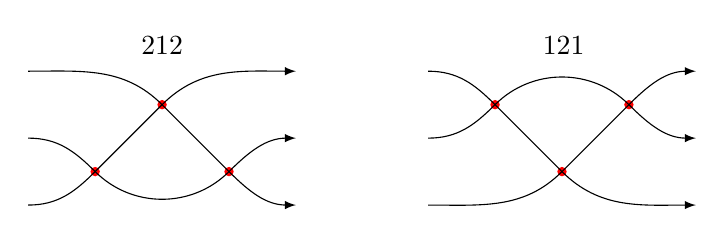
\begin{tikzpicture}[scale=0.85]
\begin{scope}[>=latex,xshift=0pt]
\draw (2,2.1) circle(0pt) node[above]{212};
\draw (8,2.1) circle(0pt) node[above]{121};
{\color{red}
\fill (1,0.5) circle(2pt) coordinate(A) node[below]{};
\fill (2,1.5) circle(2pt) coordinate(B) node[above]{};
\fill (3,0.5) circle(2pt) coordinate(C) node[below]{};
}
%
\draw [-] (0,2) to [out = 0, in = 135] (B);
\draw [-] (B) -- (C);
\draw [->] (C) to [out = -45, in = 180] (4,0);
%
\draw [-] (0,1) to [out = 0, in = 135] (A);
\draw [-] (A) to [out = -45, in = -135] (C);
\draw [->] (C) to [out = 45, in = 180] (4,1);
%
\draw [-] (0,0) to [out = 0, in = -135] (A);
\draw [-] (A) -- (B);
\draw [->] (B) to [out = 45, in = 180] (4,2);
%
\coordinate (P1) at (4.5,1);
\coordinate (P2) at (5.5,1);
%\draw[->] (P1) -- (P2);
%\draw (5,1) circle(0pt) node[below]{$R_{ABC}$};
\end{scope}
%
\begin{scope}[>=latex,xshift=170pt]
{\color{red}
\fill (3,1.5) circle(2pt) coordinate(A) node[above]{};
\fill (2,0.5) circle(2pt) coordinate(B) node[below]{};
\fill (1,1.5) circle(2pt) coordinate(C) node[above]{};
}
%
\draw [-] (0,0) to [out = 0, in = -135] (B);
\draw [-] (B) -- (A);
\draw [->] (A) to [out = 45, in = 180] (4,2);
%
\draw [-] (0,1) to [out = 0, in = -135] (C);
\draw [-] (C) to [out = 45, in = 135] (A);
\draw [->] (A) to [out = -45, in = 180] (4,1);
%
\draw [-] (0,2) to [out = 0, in = 135] (C);
\draw [-] (C) -- (B);
\draw [->] (B) to [out = -45, in = 180] (4,0);
\end{scope}
\end{tikzpicture}

\caption{Wiring diagrams for the reduced words 212 and 121 of the
 longest element $s_2s_1s_2=s_1s_2s_1$ of $W(A_2)$.}
\end{figure}

Given a wiring diagram, the associated symmetric butterfly quiver has
the vertices in the domains and on the crossings of it. The vertices
are interconnected by elementary triangles which are oriented with
dotted arrows. A pair of dotted arrows pointing in the same (resp.\
opposite) direction are regarded as a solid arrow (resp.~none). We
choose the convention that quiver vertices on the crossings of the
wiring diagram become sources vertically and sinks horizontally.

\begin{figure}[t]\centering
%\begin{align}
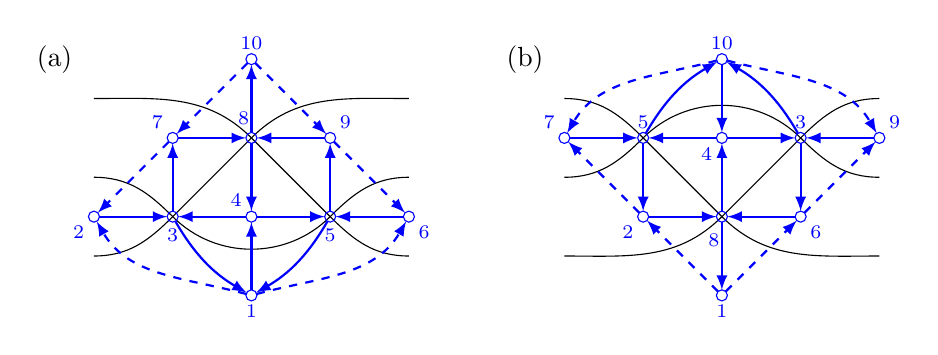
\begin{tikzpicture}
\begin{scope}[>=latex,xshift=0pt]
\draw (-0.5,2.5) node{(a)};
%
\coordinate (A) at (1,0.5);
\coordinate (B) at (2,1.5);
\coordinate (C) at (3,0.5);
%\fill (1,0.5) circle(2pt) coordinate(A);% node[below]{$A$};
%\fill (2,1.5) circle(2pt) coordinate(B);% node[above]{$B$};
%\fill (3,0.5) circle(2pt) coordinate(C);% node[below]{$C$};
%
\draw [-] (0,2) to [out = 0, in = 135] (B);
\draw [-] (B) -- (C);
\draw [-] (C) to [out = -45, in = 180] (4,0);
%
\draw [-] (0,1) to [out = 0, in = 135] (A);
\draw [-] (A) to [out = -45, in = -135] (C);
\draw [-] (C) to [out = 45, in = 180] (4,1);
%
\draw [-] (0,0) to [out = 0, in = -135] (A);
\draw [-] (A) -- (B);
\draw [-] (B) to [out = 45, in = 180] (4,2);
%
%\coordinate (P1) at (4.5,1);
%\coordinate (P2) at (5.5,1);
%\draw[->] (P1) -- (P2);
%\draw (5,1) circle(0pt) node[below]{$R_{ABC}$};
%
%
{\color{blue}
\draw (2,-0.5) circle(2pt) coordinate(1) node[below]{\scriptsize$1$};
\draw (0,0.5) circle(2pt) coordinate(2) node[below left]{\scriptsize$2$};
\draw (1,0.5) circle(2pt) coordinate(3) node[below=1pt]{\scriptsize$3$};
\draw (2,0.5) circle(2pt) coordinate(4) node[above left]{\scriptsize$4$};
\draw (3,0.5) circle(2pt) coordinate(5) node[below=1pt]{\scriptsize$5$};
\draw (4,0.5) circle(2pt) coordinate(6) node[below right]{\scriptsize$6$};
\draw (1,1.5) circle(2pt) coordinate(7) node[above left]{\scriptsize$7$};
\draw (2,1.5) circle(2pt) coordinate(8);
\draw (1.9,1.75) node {\scriptsize$8$};
\draw (3,1.5) circle(2pt) coordinate(9) node[above right]{\scriptsize$9$};
\draw (2,2.5) circle(2pt) coordinate(10) node[above]{\scriptsize$10$};
\draw[->,dashed, shorten >=2pt,shorten <=2pt] (1) to [out = 165, in = -60] (2) [thick];
%\qarrow{3}{1}
\draw[->,shorten >=2pt,shorten <=2pt] (3) to [out = -60, in = 150] (1) [thick];
\qarrow{1}{4}
\draw[->,shorten >=2pt,shorten <=2pt] (5) to [out = -120, in = 30] (1) [thick];
%\qarrow{5}{1}
%\qdarrow{1}{6}
\draw[->,dashed, shorten >=2pt,shorten <=2pt] (1) to [out = 15, in = -120] (6) [thick];
\qarrow{6}{5}
\qarrow{4}{5}
\qarrow{4}{3}
\qarrow{2}{3}
\qdarrow{7}{2}
\qarrow{3}{7}
\qarrow{8}{4}
\qarrow{5}{9}
\qdarrow{9}{6}
\qarrow{9}{8}
\qarrow{7}{8}
\qdarrow{10}{7}
\qarrow{8}{10}
\qdarrow{10}{9}
}
\end{scope}
%
\begin{scope}[>=latex,xshift=170pt]
\draw (-0.5,2.5) node{(b)};
%
\coordinate (A) at (3,1.5);
\coordinate (B) at (2,0.5);
\coordinate (C) at (1,1.5);
%\fill (3,1.5) circle(2pt) coordinate(A);% node[above]{$A$};
%\fill (2,0.5) circle(2pt) coordinate(B);% node[below]{$B$};
%\fill (1,1.5) circle(2pt) coordinate(C);% node[above]{$C$};
%
\draw [-] (0,0) to [out = 0, in = -135] (B);
\draw [-] (B) -- (A);
\draw [-] (A) to [out = 45, in = 180] (4,2);
%
\draw [-] (0,1) to [out = 0, in = -135] (C);
\draw [-] (C) to [out = 45, in = 135] (A);
\draw [-] (A) to [out = -45, in = 180] (4,1);
%
\draw [-] (0,2) to [out = 0, in = 135] (C);
\draw [-] (C) -- (B);
\draw [-] (B) to [out = -45, in = 180] (4,0);
%
%
{\color{blue}
\draw (2,-0.5) circle(2pt) coordinate(1) node[below]{\scriptsize$1$};
\draw (1,0.5) circle(2pt) coordinate(2) node[below left]{\scriptsize$2$};
\draw (3,1.5) circle(2pt) coordinate(3) node[above]{\scriptsize$3$};
\draw (2,1.5) circle(2pt) coordinate(4) node[below left]{\scriptsize$4$};
\draw (1,1.5) circle(2pt) coordinate(5) node[above]{\scriptsize$5$};
\draw (3,0.5) circle(2pt) coordinate(6) node[below right]{\scriptsize$6$};
\draw (0,1.5) circle(2pt) coordinate(7) node[above left]{\scriptsize$7$};
\draw (2,0.5) circle(2pt) coordinate(8);
\draw (1.9,0.2) node {\scriptsize$8$};
\draw (4,1.5) circle(2pt) coordinate(9) node[above right]{\scriptsize$9$};
\draw (2,2.5) circle(2pt) coordinate(10) node[above]{\scriptsize$10$};
%
\draw[->,dashed, shorten >=2pt,shorten <=2pt] (10) to [out = -165, in = 60] (7) [thick];
\draw[->,shorten >=2pt,shorten <=2pt] (5) to [out = 60, in = -150] (10) [thick];\qarrow{10}{4}
\draw[->,shorten >=2pt,shorten <=2pt] (3) to [out = 120, in = -30] (10) [thick];
\draw[->,dashed, shorten >=2pt,shorten <=2pt] (10) to [out = -15, in = 120] (9) [thick];
\qarrow{7}{5}
\qarrow{4}{5}
\qarrow{4}{3}
\qarrow{9}{3}
\qdarrow{2}{7}
\qarrow{8}{4}
\qarrow{5}{2}
\qarrow{3}{6}
\qdarrow{6}{9}
\qarrow{2}{8}
\qarrow{6}{8}
\qdarrow{1}{2}
\qarrow{8}{1}
\qdarrow{1}{6}
}
\end{scope}
\end{tikzpicture}

\vspace{-3mm}
\caption{Symmetric butterfly quivers (depicted in blue) associated
 with the wiring diagrams. Given the labels $1,\dotsc, 10$ of the
 quiver vertices in (a), those in (b) are determined following the
 mutation sequence in Figure \ref{fig:mus}.}\label{fig:3.2}\vspace{-2mm}
\end{figure}



\begin{Remark}\label{re:c1}
 Let $B$ be the exchange matrix corresponding to the symmetric
 butterfly quiver in Figure \ref{fig:3.2}\,(a). Then the skew filed
 $\mathcal{Y}(B)$ generated by $Y_1, \dots, Y_{10}$ has the center
 generated by
\[
Y^{-1}_1Y_7Y_8Y_9Y^2_{10},\qquad
Y_2Y^{-1}_4Y_6Y_{10},\qquad
Y_3Y^2_4Y^{-2}_6Y^2_7Y_8,\qquad
Y_5Y^2_6Y_8Y^2_9Y^2_{10}.
\]


\end{Remark}

\subsection[Cluster transformation R]{Cluster transformation $\boldsymbol{\widehat{R}}$}

Let $\bigl(B^{(1)}, \bY^{(1)}\bigr) = (B, \bY)$ and
$\bigl(B^{(6)}, \bY^{(6)}\bigr) = \bigl(B', \bY'\bigr)$ be the quantum $y$-seeds corresponding to Figure \ref{fig:3.2}\,(a) and (b), respectively.
We connect them by the following mutation sequence
%
\begin{align}
\bigl(B^{(1)}, \bY^{(1)}\bigr) &\underset{\varepsilon_1}{\overset{\mu_4}{\longleftrightarrow}}
\bigl(B^{(2)}, \bY^{(2)}\bigr) \underset{\varepsilon_2}{\overset{\mu_3}{\longleftrightarrow}}
\bigl(B^{(3)}, \bY^{(3)}\bigr)\nonumber
\\
&\underset{\varepsilon_3}{\overset{\mu_5}{\longleftrightarrow}}
\bigl(B^{(4)}, \bY^{(4)}\bigr) \underset{\varepsilon_4}{\overset{\mu_8}{\longleftrightarrow}}
\bigl(B^{(5)}, \bY^{(5)}\bigr) \overset{\sigma_{3,5}\sigma_{4,8}}{\longleftrightarrow}
\bigl(B^{(6)}, \bY^{(6)}\bigr),\label{mus}
\end{align}
where \smash{$\bY^{(t)}=\bigl(Y^{(t)}_1,\dotsc, Y^{(t)}_{10}\bigr)$}. The symbol
$\sigma_{ij}$ denotes the exchange of the indices $i$ and $j$ in the
exchange matrix and $Y$-variables. See \eqref{qys}. We have also
attached the signs $\varepsilon_i=\pm 1$ along which the decomposition
\eqref{mud} into the automorphism part and the monomial part will be
considered. See Figure \ref{fig:mus}.

\begin{figure}[t]\centering
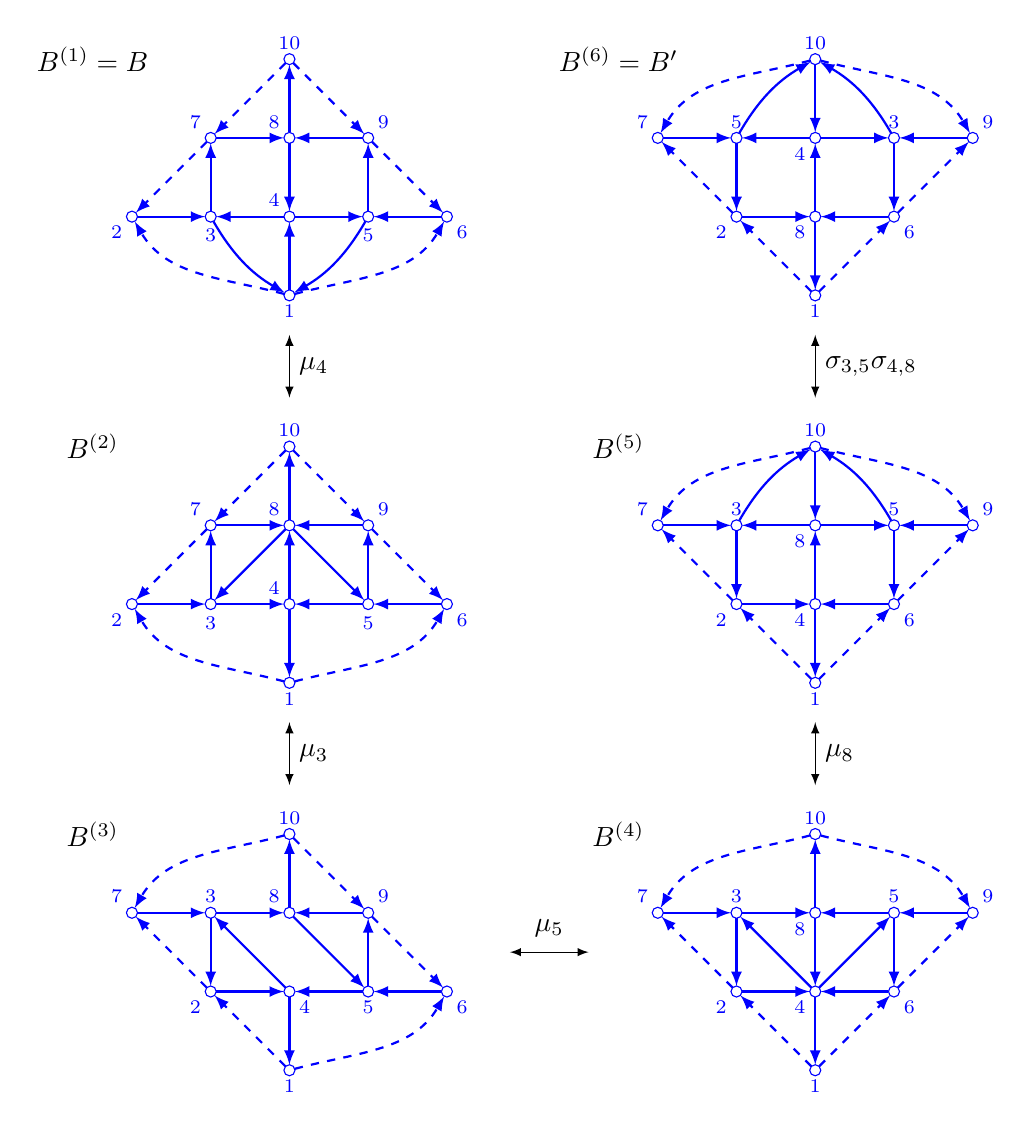
\begin{tikzpicture}
\begin{scope}[>=latex,xshift=0pt]
\draw (-0.5,2.5) node{$B^{(1)}=B$};
%
{\color{blue}
\draw (2,-0.5) circle(2pt) coordinate(1) node[below]{\scriptsize$1$};
\draw (0,0.5) circle(2pt) coordinate(2) node[below left]{\scriptsize$2$};
\draw (1,0.5) circle(2pt) coordinate(3) node[below=1pt]{\scriptsize$3$};
\draw (2,0.5) circle(2pt) coordinate(4) node[above left]{\scriptsize$4$};
\draw (3,0.5) circle(2pt) coordinate(5) node[below=1pt]{\scriptsize$5$};
\draw (4,0.5) circle(2pt) coordinate(6) node[below right]{\scriptsize$6$};
\draw (1,1.5) circle(2pt) coordinate(7) node[above left]{\scriptsize$7$};
\draw (2,1.5) circle(2pt) coordinate(8) node[above left]{\scriptsize$8$};
\draw (3,1.5) circle(2pt) coordinate(9) node[above right]{\scriptsize$9$};
\draw (2,2.5) circle(2pt) coordinate(10) node[above]{\scriptsize$10$};
\draw[->,dashed, shorten >=2pt,shorten <=2pt] (1) to [out = 165, in = -60] (2) [thick];
\draw[->,shorten >=2pt,shorten <=2pt] (3) to [out = -60, in = 150] (1) [thick];
\qarrow{1}{4}
\draw[->,shorten >=2pt,shorten <=2pt] (5) to [out = -120, in = 30] (1) [thick];
\draw[->,dashed, shorten >=2pt,shorten <=2pt] (1) to [out = 15, in = -120] (6) [thick];
\qarrow{6}{5}
\qarrow{4}{5}
\qarrow{4}{3}
\qarrow{2}{3}
\qdarrow{7}{2}
\qarrow{3}{7}
\qarrow{8}{4}
\qarrow{5}{9}
\qdarrow{9}{6}
\qarrow{9}{8}
\qarrow{7}{8}
\qdarrow{10}{7}
\qarrow{8}{10}
\qdarrow{10}{9}
}
%
\draw[<->] (2,-1) -- (2,-1.8);
\draw (2,-1.4) node[right] {$\mu_4$};
\end{scope}
%
\begin{scope}[>=latex,xshift=190pt]
\draw (-0.5,2.5) node{$B^{(6)}=B'$};
%
{\color{blue}
\draw (2,-0.5) circle(2pt) coordinate(1) node[below]{\scriptsize$1$};
\draw (1,0.5) circle(2pt) coordinate(2) node[below left]{\scriptsize$2$};
\draw (3,1.5) circle(2pt) coordinate(3) node[above]{\scriptsize$3$};
\draw (2,1.5) circle(2pt) coordinate(4) node[below left]{\scriptsize$4$};
\draw (1,1.5) circle(2pt) coordinate(5) node[above]{\scriptsize$5$};
\draw (3,0.5) circle(2pt) coordinate(6) node[below right]{\scriptsize$6$};
\draw (0,1.5) circle(2pt) coordinate(7) node[above left]{\scriptsize$7$};
\draw (2,0.5) circle(2pt) coordinate(8) node[below left]{\scriptsize$8$};
%\draw (1.9,0.2) node {\scriptsize$8$};
\draw (4,1.5) circle(2pt) coordinate(9) node[above right]{\scriptsize$9$};
\draw (2,2.5) circle(2pt) coordinate(10) node[above]{\scriptsize$10$};
%
\draw[->,dashed, shorten >=2pt,shorten <=2pt] (10) to [out = -165, in = 60] (7) [thick];
\draw[->,shorten >=2pt,shorten <=2pt] (5) to [out = 60, in = -150] (10) [thick];\qarrow{10}{4}
\draw[->,shorten >=2pt,shorten <=2pt] (3) to [out = 120, in = -30] (10) [thick];
\draw[->,dashed, shorten >=2pt,shorten <=2pt] (10) to [out = -15, in = 120] (9) [thick];
\qarrow{7}{5}
\qarrow{4}{5}
\qarrow{4}{3}
\qarrow{9}{3}
\qdarrow{2}{7}
\qarrow{8}{4}
\qarrow{5}{2}
\qarrow{3}{6}
\qdarrow{6}{9}
\qarrow{2}{8}
\qarrow{6}{8}
\qdarrow{1}{2}
\qarrow{8}{1}
\qdarrow{1}{6}
}
\draw[<->] (2,-1) -- (2,-1.8);
\draw (2,-1.4) node[right] {$\sigma_{3,5} \sigma_{4,8}$};
\end{scope}
%
\begin{scope}[>=latex,xshift=0pt,yshift=-140pt]
\draw (-0.5,2.5) node{$B^{(2)}$};
%
{\color{blue}
\draw (2,-0.5) circle(2pt) coordinate(1) node[below]{\scriptsize$1$};
\draw (0,0.5) circle(2pt) coordinate(2) node[below left]{\scriptsize$2$};
\draw (1,0.5) circle(2pt) coordinate(3) node[below=1pt]{\scriptsize$3$};
\draw (2,0.5) circle(2pt) coordinate(4) node[above left]{\scriptsize$4$};
\draw (3,0.5) circle(2pt) coordinate(5) node[below=1pt]{\scriptsize$5$};
\draw (4,0.5) circle(2pt) coordinate(6) node[below right]{\scriptsize$6$};
\draw (1,1.5) circle(2pt) coordinate(7) node[above left]{\scriptsize$7$};
\draw (2,1.5) circle(2pt) coordinate(8) node[above left]{\scriptsize$8$};
\draw (3,1.5) circle(2pt) coordinate(9) node[above right]{\scriptsize$9$};
\draw (2,2.5) circle(2pt) coordinate(10) node[above]{\scriptsize$10$};
\draw[->,dashed, shorten >=2pt,shorten <=2pt] (1) to [out = 165, in = -60] (2) [thick];
\qarrow{4}{1}
\draw[->,dashed, shorten >=2pt,shorten <=2pt] (1) to [out = 15, in = -120] (6) [thick];
\qarrow{6}{5}
\qarrow{5}{4}
\qarrow{3}{4}
\qarrow{2}{3}
\qdarrow{7}{2}
\qarrow{3}{7}
\qarrow{8}{3}
\qarrow{4}{8}
\qarrow{8}{5}
\qarrow{5}{9}
\qdarrow{9}{6}
\qarrow{9}{8}
\qarrow{7}{8}
\qdarrow{10}{7}
\qarrow{8}{10}
\qdarrow{10}{9}
}
%
\draw[<->] (2,-1) -- (2,-1.8);
\draw (2,-1.4) node[right] {$\mu_3$};
\end{scope}
%
\begin{scope}[>=latex,xshift=190pt,yshift=-140pt]
\draw (-0.5,2.5) node{$B^{(5)}$};
%
{\color{blue}
\draw (2,-0.5) circle(2pt) coordinate(1) node[below]{\scriptsize$1$};
\draw (1,0.5) circle(2pt) coordinate(2) node[below left]{\scriptsize$2$};
\draw (3,1.5) circle(2pt) coordinate(3) node[above]{\scriptsize$5$};
\draw (2,1.5) circle(2pt) coordinate(4) node[below left]{\scriptsize$8$};
\draw (1,1.5) circle(2pt) coordinate(5) node[above]{\scriptsize$3$};
\draw (3,0.5) circle(2pt) coordinate(6) node[below right]{\scriptsize$6$};
\draw (0,1.5) circle(2pt) coordinate(7) node[above left]{\scriptsize$7$};
\draw (2,0.5) circle(2pt) coordinate(8) node[below left]{\scriptsize$4$};
\draw (4,1.5) circle(2pt) coordinate(9) node[above right]{\scriptsize$9$};
\draw (2,2.5) circle(2pt) coordinate(10) node[above]{\scriptsize$10$};
%
\draw[->,dashed, shorten >=2pt,shorten <=2pt] (10) to [out = -165, in = 60] (7) [thick];
\draw[->,shorten >=2pt,shorten <=2pt] (5) to [out = 60, in = -150] (10) [thick];\qarrow{10}{4}
\draw[->,shorten >=2pt,shorten <=2pt] (3) to [out = 120, in = -30] (10) [thick];
\draw[->,dashed, shorten >=2pt,shorten <=2pt] (10) to [out = -15, in = 120] (9) [thick];
\qarrow{7}{5}
\qarrow{4}{5}
\qarrow{4}{3}
\qarrow{9}{3}
\qdarrow{2}{7}
\qarrow{8}{4}
\qarrow{5}{2}
\qarrow{3}{6}
\qdarrow{6}{9}
\qarrow{2}{8}
\qarrow{6}{8}
\qdarrow{1}{2}
\qarrow{8}{1}
\qdarrow{1}{6}
}
\draw[<->] (2,-1) -- (2,-1.8);
\draw (2,-1.4) node[right] {$\mu_8$};
\end{scope}
%
\begin{scope}[>=latex,xshift=0pt,yshift=-280pt]
\draw (-0.5,2.5) node{$B^{(3)}$};
%
{\color{blue}
\draw (2,-0.5) circle(2pt) coordinate(1) node[below]{\scriptsize$1$};
\draw (1,0.5) circle(2pt) coordinate(2) node[below left]{\scriptsize$2$};
\draw (1,1.5) circle(2pt) coordinate(3) node[above]{\scriptsize$3$};
\draw (2,0.5) circle(2pt) coordinate(4) node[below right]{\scriptsize$4$};
\draw (3,0.5) circle(2pt) coordinate(5) node[below]{\scriptsize$5$};
\draw (4,0.5) circle(2pt) coordinate(6) node[below right]{\scriptsize$6$};
\draw (0,1.5) circle(2pt) coordinate(7) node[above left]{\scriptsize$7$};
\draw (2,1.5) circle(2pt) coordinate(8) node[above left]{\scriptsize$8$};
\draw (3,1.5) circle(2pt) coordinate(9) node[above right]{\scriptsize$9$};
\draw (2,2.5) circle(2pt) coordinate(10) node[above]{\scriptsize$10$};
%
\qdarrow{1}{2}
%\draw[->,dashed, shorten >=2pt,shorten <=2pt] (1) to [out = 165, in = -60] (2) [thick];
\qarrow{4}{1}
\draw[->,dashed, shorten >=2pt,shorten <=2pt] (1) to [out = 15, in = -120] (6) [thick];;
\qarrow{6}{5}
\qarrow{5}{4}
\qarrow{2}{4}
%\qarrow{2}{3}
\qdarrow{2}{7}
\qarrow{3}{2}
\qarrow{4}{3}
%\qarrow{4}{8}
\qarrow{8}{5}
\qarrow{5}{9}
\qdarrow{9}{6}
\qarrow{7}{3}
\qarrow{3}{8}
\qarrow{9}{8}
\draw[->,dashed, shorten >=2pt,shorten <=2pt] (10) to [out = -165, in = 60] (7) [thick];
%\qdarrow{10}{7}
\qarrow{8}{10}
\qdarrow{10}{9}
}
%
\draw[<->] (4.8,1) -- (5.8,1);
\draw (5.3,1.3) node {$\mu_5$};
\end{scope}
%
\begin{scope}[>=latex,xshift=190pt,yshift=-280pt]
\draw (-0.5,2.5) node{$B^{(4)}$};
%
{\color{blue}
\draw (2,-0.5) circle(2pt) coordinate(1) node[below]{\scriptsize$1$};
\draw (1,0.5) circle(2pt) coordinate(2) node[below left]{\scriptsize$2$};
\draw (3,1.5) circle(2pt) coordinate(3) node[above]{\scriptsize$5$};
\draw (2,1.5) circle(2pt) coordinate(4) node[below left]{\scriptsize$8$};
\draw (1,1.5) circle(2pt) coordinate(5) node[above]{\scriptsize$3$};
\draw (3,0.5) circle(2pt) coordinate(6) node[below right]{\scriptsize$6$};
\draw (0,1.5) circle(2pt) coordinate(7) node[above left]{\scriptsize$7$};
\draw (2,0.5) circle(2pt) coordinate(8) node[below left]{\scriptsize$4$};
\draw (4,1.5) circle(2pt) coordinate(9) node[above right]{\scriptsize$9$};
\draw (2,2.5) circle(2pt) coordinate(10) node[above]{\scriptsize$10$};
%
\draw[->,dashed, shorten >=2pt,shorten <=2pt] (10) to [out = -165, in = 60] (7) [thick];
%\draw[->,shorten >=2pt,shorten <=2pt] (5) to [out = 60, in = -150] (10) [thick];\qarrow{4}{10}
%\draw[->,shorten >=2pt,shorten <=2pt] (3) to [out = 120, in = -30] (10) [thick];
\draw[->,dashed, shorten >=2pt,shorten <=2pt] (10) to [out = -15, in = 120] (9) [thick];
\qarrow{4}{10}
\qarrow{7}{5}
\qarrow{5}{4}
\qarrow{3}{4}
\qarrow{9}{3}
\qdarrow{2}{7}
\qarrow{4}{8}
\qarrow{8}{5}
\qarrow{8}{3}
\qarrow{5}{2}
\qarrow{3}{6}
\qdarrow{6}{9}
\qarrow{2}{8}
\qarrow{6}{8}
\qdarrow{1}{2}
\qarrow{8}{1}
\qdarrow{1}{6}
}
\end{scope}
\end{tikzpicture}
%\vspace*{-3.5cm}
%\hspace*{-1.1cm}
%\includegraphics[clip,scale=0.55]{FIG3.3.pdf}
%\vspace*{-2.2cm}
\caption{The quivers $B=B^{(1)}, \dots, B^{(6)}=B'$ and the
 mutations connecting them. We do not consider the wiring diagrams
 corresponding to the intermediate ones $B^{(2)}, \dots, B^{(5)}$.}
\label{fig:mus}
\end{figure}

For simplicity, we identify \smash{$Y^{(t)}_i$} and $\rY_i(t)$ in the
description from now on. We introduce the cluster transformation
\smash{$\widehat{R}\colon \mathcal{Y}\bigl(B'\bigr) \rightarrow \mathcal{Y}(B)$}
corresponding to the mutation sequence \eqref{mus} by applying
\eqref{yad} as
\begin{align}
\widehat{R} ={}&
\mathrm{Ad}\bigl(\Psi_q\bigl(\bigl(Y^{(1)}_4\bigr)^{\varepsilon_1}\bigr)^{\varepsilon_1}\bigr)\tau_{4,\varepsilon_1}
\mathrm{Ad}\bigl(\Psi_q\bigl(\bigl(Y^{(2)}_3\bigr)^{\varepsilon_2}\bigr)^{\varepsilon_2}\bigr)\tau_{3,\varepsilon_2}\nonumber
\\
 & \times
\mathrm{Ad}\bigl(\Psi_q\bigl(\bigl(Y^{(3)}_5\bigr)^{\varepsilon_3}\bigr)^{\varepsilon_3}\bigr)\tau_{5,\varepsilon_3}
\mathrm{Ad}\bigl(\Psi_q\bigl(\bigl(Y^{(4)}_8\bigr)^{\varepsilon_4}\bigr)^{\varepsilon_4}\bigr)\tau_{8,\varepsilon_4}
\sigma_{3,5}\sigma_{4,8}.\label{rhat}
\end{align}
The selection of $(\varepsilon_1, \varepsilon_2, \varepsilon_3, \varepsilon_4) \in \{1,-1\}^4$
influences the expressions, but \smash{$\widehat{R}$} itself remains independent of it.
We set
\begin{align}\label{taue}
\tau_{\varepsilon_1, \varepsilon_2, \varepsilon_3, \varepsilon_4} =
\tau_{4,\varepsilon_1}
\tau_{3,\varepsilon_2}
\tau_{5,\varepsilon_3}
\tau_{8,\varepsilon_4} \sigma_{3,5}\sigma_{4,8}\colon\
\mathcal{Y}\bigl(B'\bigr) \rightarrow \mathcal{Y}(B),
 \end{align}
 and call it the monomial part of \smash{$\widehat{R}$}.


\begin{Example}\label{ex:1}
$\tau_{--++}$ and $\tau_{--++}^{-1}$ are given as follows:
\begin{align*}
&\tau_{--++}\colon\
\begin{cases}
Y'_1 \mapsto Y_1,\qquad
Y'_2 \mapsto Y_2, \qquad
Y'_3 \mapsto Y_8, \qquad
Y'_4 \mapsto Y^{-1}_4Y^{-1}_5Y^{-1}_8, \qquad
\\
Y'_5 \mapsto Y^{-1}_3Y_5Y_8, \qquad
Y'_6 \mapsto Y_4 Y_5 Y_6,\qquad
Y'_7 \mapsto Y_3Y_4Y_7,\qquad
Y'_8 \mapsto Y_3,\qquad
\\
Y'_9 \mapsto Y_9, \qquad
Y'_{10} \mapsto Y_{10},
\end{cases}
\\
&\tau_{--++}^{-1}\colon\
\begin{cases}
Y_1 \mapsto Y'_1, \qquad
Y_2 \mapsto Y'_2, \qquad
Y_3 \mapsto Y'_8, \qquad
Y_4 \mapsto Y'^{-1}_4Y'^{-1}_5Y'^{-1}_8,
\\
Y_5 \mapsto Y'^{-1}_3Y'_5Y'_8, \qquad
Y_6 \mapsto Y'_3Y'_4Y'_6, \qquad
Y_7 \mapsto Y'_4Y'_5Y'_7, \qquad
Y_8 \mapsto Y'_3,
\\
Y_9 \mapsto Y'_9, \qquad
Y_{10} \mapsto Y'_{10}.
\end{cases}
\end{align*}
By using them, $\widehat{R}$ in \eqref{rhat} for the choice
$(\varepsilon_1, \varepsilon_2, \varepsilon_3, \varepsilon_4)=(-,-,+,+)$
is expressed as
\begin{align}
\widehat{R}={}&
\mathrm{Ad}\bigl(\Psi_q\bigl(\bigl(Y^{(1)}_4\bigr)^{-1}\bigr)^{-1}\bigr)\tau_{4,-}
\mathrm{Ad}\bigl(\Psi_q\bigl(\bigl(Y^{(2)}_3\bigr)^{-1}\bigr)^{-1}\bigr)\tau_{3,-}
\nonumber \\
& \times
\mathrm{Ad}\bigl(\Psi_q\bigl(Y^{(3)}_5\bigr)\bigr)\tau_{5,+}
 \mathrm{Ad}\bigl(\Psi_q\bigl(Y^{(4)}_8\bigr)\bigr)\tau_{8,+}\sigma_{3,5}\sigma_{4,8}
\nonumber \\
={}&
\mathrm{Ad}\bigl(\Psi_q\bigl(Y_4^{-1}\bigr)^{-1}
\Psi_q\bigl(qY^{-1}_3Y^{-1}_4\bigr)^{-1}
\Psi_q\bigl(q^{-1}Y_4Y_5\bigr)
\Psi_q\bigl(Y_4Y_5Y_8\bigr)\bigr)\tau_{--++}
\label{dode0}\\
={}&
\mathrm{Ad}\bigl(
\Psi_q\bigl(Y_4^{-1}\bigr)^{-1}
\Psi_q\bigl(qY^{-1}_3Y^{-1}_4\bigr)^{-1}\bigr)
\tau_{--++}
\mathrm{Ad}\bigl(
\Psi_q\bigl(qY'^{-1}_3Y'^{-1}_4\bigr)
\Psi_q\bigl(Y'^{-1}_4\bigr)\bigr).
\label{dode}
\end{align}
The formula \eqref{dode} is derived from \eqref{dode0}
by moving $\tau_{--++}$ to the left by using $\tau_{--++}^{-1}$.
\end{Example}

\begin{Example}\label{ex:2}
$\tau_{-+-+}$ and $\tau_{-+-+}^{-1}$ are given as follows:
\begin{align*}
&\tau_{-+-+}\colon\
\begin{cases}
Y'_1 \mapsto Y_1,\qquad
Y'_2 \mapsto Y_2Y_3Y_4, \qquad
Y'_3 \mapsto Y_3Y^{-1}_5Y_8, \qquad
Y'_4 \mapsto q^2Y^{-1}_3Y^{-1}_4Y^{-1}_8,
\\
Y'_5 \mapsto Y_8, \qquad
Y'_6 \mapsto Y_6,\qquad
Y'_7 \mapsto Y_7,\qquad
Y'_8 \mapsto Y_5,
\\
Y'_9 \mapsto q^{-2}Y_4Y_5Y_9, \qquad
Y'_{10} \mapsto Y_{10},
\end{cases}
\\
& \tau_{-+-+}^{-1}\colon\
\begin{cases}
Y_1 \mapsto Y'_1, \qquad\!
Y_2 \mapsto Y'_2Y'_4Y'_5, \qquad\!
Y_3 \mapsto Y'_3Y'^{-1}_5Y'_8, \qquad\!
Y_4 \mapsto q^2Y'^{-1}_3Y'^{-1}_4Y'^{-1}_8,
\\
Y_5 \mapsto Y'_8, \qquad
Y_6 \mapsto Y'_6, \qquad
Y_7 \mapsto Y'_7, \qquad
Y_8 \mapsto Y'_5,
\\
Y_9 \mapsto q^2Y'_3Y'_4Y'_9, \qquad
Y_{10} \mapsto Y'_{10}.
\end{cases}
\end{align*}
By using them, $\widehat{R}$ in \eqref{rhat} for the choice
$(\varepsilon_1, \varepsilon_2, \varepsilon_3, \varepsilon_4)=(-,+,-,+)$
is expressed as
\begin{align}
\widehat{R}={}&
\mathrm{Ad}\bigl(\Psi_q\bigl(\bigl(Y^{(1)}_4\bigr)^{-1}\bigr)^{-1}\bigr)\tau_{4,-}
\mathrm{Ad}\bigl(\Psi_q\bigl(Y^{(2)}_3\bigr)\bigr)\tau_{3,+}
\nonumber \\
& \times
\mathrm{Ad}\bigl(\Psi_q\bigl(\bigl(Y^{(3)}_5\bigr)^{-1}\bigr)^{-1}\bigr)\tau_{5,-}
\mathrm{Ad}\bigl(\Psi_q\bigl(Y^{(4)}_8\bigr)\bigr)\tau_{8,+}\sigma_{3,5}\sigma_{4,8}
\nonumber \\
={}&
\mathrm{Ad}\bigl(\Psi_q\bigl(Y_4^{-1}\bigr)^{-1}
\Psi_q(qY_3Y_4)
\Psi_q\bigl(qY^{-1}_5Y^{-1}_4\bigr)^{-1}
\Psi_q\bigl(q^2Y_3Y_4Y_8\bigr)\bigr)\tau_{-+-+}
\label{dode1}\\
={}&
\mathrm{Ad}\bigl(
\Psi_q\bigl(Y_4^{-1}\bigr)^{-1}
\Psi_q(qY_3Y_4)^{-1}\bigr)
\tau_{-+-+}
\mathrm{Ad}\bigl(
\Psi_q(qY'_3Y'_4)^{-1}
\Psi_q\bigl(Y'^{-1}_4\bigr)\bigr).
\label{dode2}
\end{align}
\end{Example}

Performing a straightforward calculation using any one
of the formulas for $\widehat{R}$ in Examples~\ref{ex:1} and \ref{ex:2},
we get the following.

\begin{Proposition}\label{pr:RY}
The cluster transformation $\widehat{R}\colon \mathcal{Y}\bigl(B'\bigr) \rightarrow \mathcal{Y}(B)$ is given by
\begin{gather*}
Y'_1 \mapsto q\Lambda^{-1}_4Y_4Y_1,\qquad
Y'_2 \mapsto qY_3\Lambda_4\Lambda^{-1}_3Y_2,
\qquad
Y'_3 \mapsto q^2 \Lambda^{-1}_0Y_3Y_4Y_8,
\\
Y'_4 \mapsto q\Lambda^{-1}_4Y^{-1}_3Y^{-1}_4Y^{-1}_5Y^{-1}_8\Lambda_3\Lambda_5,
\qquad
Y'_5 \mapsto \Lambda^{-1}_0 Y_4Y_5Y_8,
\qquad
Y'_6 \mapsto q Y_5 \Lambda_4\Lambda^{-1}_5Y_6,
\\
Y'_7 \mapsto Y_7\Lambda_3,
\qquad
Y'_8 \mapsto Y^{-1}_4\Lambda_0,
\qquad
Y'_9 \mapsto Y_9\Lambda_5,
\qquad
Y'_{10} \mapsto Y_{10}\Lambda^{-1}_5\Lambda^{-1}_3\Lambda_0,
\end{gather*}
where $\Lambda_0$, $\Lambda_3$, $\Lambda_4$ and $\Lambda_5$ are given
as follows:
\begin{gather*}
\Lambda_0 = \Lambda_3\Lambda_5 + Y_4Y_3Y_5Y_8\Lambda_4,\qquad
\Lambda_3 = 1+qY_3+Y_4Y_3,\qquad
\Lambda_4 = 1 + q Y_4, \\
\Lambda_5 = 1+qY_5+Y_4Y_5.
\end{gather*}
\end{Proposition}

\begin{Remark}\label{re:c2}
$\widehat{R}$ preserves the following combinations:
\begin{gather*}
\widehat{R}\bigl(Y'_3Y'_8\bigr) = Y_3Y_8,
\qquad
\widehat{R}\bigl(Y'_5Y'_8\bigr) = Y_5Y_8,
\\
\widehat{R}\bigl(Y'_1Y'_2Y'_4Y'_6Y'_7Y'^{-1}_8Y'_9Y'_{10}\bigr) =
Y_1Y_2Y_4Y_6Y_7Y^{-1}_8Y_9Y_{10}.
\end{gather*}
\end{Remark}

\subsection[R satisfies the tetrahedron equation]{$\boldsymbol{\widehat{R}}$ satisfies the tetrahedron equation}

In the situation in Figure \ref{fig:R123}, $\widehat{R}$ is a
transformation of the 10 variables $\{Y'_1,\dotsc, Y'_{10}\}$ into
$\{Y_1,\dotsc, Y_{10}\}$ as in Proposition \ref{pr:RY}. We denote it
simply by $\widehat{R}_{123}$, where the indices $1$, $2$, $3$ are the
vertices $1$, $2$, $3$ of the wiring diagram (highlighted in red).

\begin{figure}[t]\centering
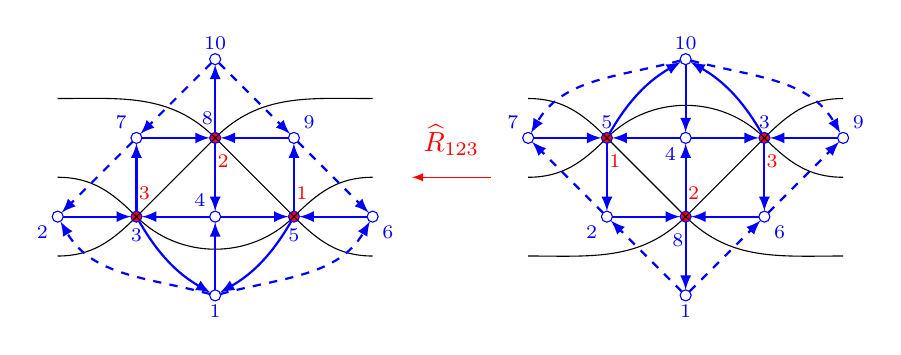
\begin{tikzpicture}
\begin{scope}[>=latex,xshift=0pt]
{\color{red}
\fill (1,0.5) circle(2pt) coordinate(A);
\draw (1.1,0.8) node {\scriptsize$3$};
\fill (2,1.5) circle(2pt) coordinate(B);
\draw (2.1,1.2) node {\scriptsize$2$};
\fill (3,0.5) circle(2pt) coordinate(C);
\draw (3.1,0.8) node {\scriptsize$1$};
}
%
\draw [-] (0,2) to [out = 0, in = 135] (B);
\draw [-] (B) -- (C);
\draw [-] (C) to [out = -45, in = 180] (4,0);
%
\draw [-] (0,1) to [out = 0, in = 135] (A);
\draw [-] (A) to [out = -45, in = -135] (C);
\draw [-] (C) to [out = 45, in = 180] (4,1);
%
\draw [-] (0,0) to [out = 0, in = -135] (A);
\draw [-] (A) -- (B);
\draw [-] (B) to [out = 45, in = 180] (4,2);
%
{\color{red}
\coordinate (P1) at (4.5,1);
\coordinate (P2) at (5.5,1);
\draw[->] (5.5,1) -- (4.5,1);
\draw (5,1.8) circle(0pt) node[below]{$\widehat{R}_{123}$};
}
%
%
{\color{blue}
\draw (2,-0.5) circle(2pt) coordinate(1) node[below]{\scriptsize$1$};
\draw (0,0.5) circle(2pt) coordinate(2) node[below left]{\scriptsize$2$};
\draw (1,0.5) circle(2pt) coordinate(3) node[below=1pt]{\scriptsize$3$};
\draw (2,0.5) circle(2pt) coordinate(4) node[above left]{\scriptsize$4$};
\draw (3,0.5) circle(2pt) coordinate(5) node[below=1pt]{\scriptsize$5$};
\draw (4,0.5) circle(2pt) coordinate(6) node[below right]{\scriptsize$6$};
\draw (1,1.5) circle(2pt) coordinate(7) node[above left]{\scriptsize$7$};
\draw (2,1.5) circle(2pt) coordinate(8);
\draw (1.9,1.75) node {\scriptsize$8$};
\draw (3,1.5) circle(2pt) coordinate(9) node[above right]{\scriptsize$9$};
\draw (2,2.5) circle(2pt) coordinate(10) node[above]{\scriptsize$10$};
%
%\qdarrow{1}{2}
\draw[->,dashed, shorten >=2pt,shorten <=2pt] (1) to [out = 165, in = -60] (2) [thick];
%\qarrow{3}{1}
\draw[->,shorten >=2pt,shorten <=2pt] (3) to [out = -60, in = 150] (1) [thick];
\qarrow{1}{4}
\draw[->,shorten >=2pt,shorten <=2pt] (5) to [out = -120, in = 30] (1) [thick];
%\qarrow{5}{1}
%\qdarrow{1}{6}
\draw[->,dashed, shorten >=2pt,shorten <=2pt] (1) to [out = 15, in = -120] (6) [thick];
\qarrow{6}{5}
\qarrow{4}{5}
\qarrow{4}{3}
\qarrow{2}{3}
\qdarrow{7}{2}
\qarrow{3}{7}
\qarrow{8}{4}
\qarrow{5}{9}
\qdarrow{9}{6}
\qarrow{9}{8}
\qarrow{7}{8}
\qdarrow{10}{7}
\qarrow{8}{10}
\qdarrow{10}{9}
}
\end{scope}
%
\begin{scope}[>=latex,xshift=170pt]
{\color{red}
\fill (3,1.5) circle(2pt) coordinate(A);
\draw (3.1,1.2) node {\scriptsize$3$};
\fill (2,0.5) circle(2pt) coordinate(B);
\draw (2.1,0.8) node {\scriptsize$2$};
\fill (1,1.5) circle(2pt) coordinate(C);
\draw (1.1,1.2) node {\scriptsize$1$};
}
%
\draw [-] (0,0) to [out = 0, in = -135] (B);
\draw [-] (B) -- (A);
\draw [-] (A) to [out = 45, in = 180] (4,2);
%
\draw [-] (0,1) to [out = 0, in = -135] (C);
\draw [-] (C) to [out = 45, in = 135] (A);
\draw [-] (A) to [out = -45, in = 180] (4,1);
%
\draw [-] (0,2) to [out = 0, in = 135] (C);
\draw [-] (C) -- (B);
\draw [-] (B) to [out = -45, in = 180] (4,0);
%
%
{\color{blue}
\draw (2,-0.5) circle(2pt) coordinate(1) node[below]{\scriptsize$1$};
\draw (1,0.5) circle(2pt) coordinate(2) node[below left]{\scriptsize$2$};
\draw (3,1.5) circle(2pt) coordinate(3) node[above]{\scriptsize$3$};
\draw (2,1.5) circle(2pt) coordinate(4) node[below left]{\scriptsize$4$};
\draw (1,1.5) circle(2pt) coordinate(5) node[above]{\scriptsize$5$};
\draw (3,0.5) circle(2pt) coordinate(6) node[below right]{\scriptsize$6$};
\draw (0,1.5) circle(2pt) coordinate(7) node[above left]{\scriptsize$7$};
\draw (2,0.5) circle(2pt) coordinate(8);
\draw (1.9,0.2) node {\scriptsize$8$};
\draw (4,1.5) circle(2pt) coordinate(9) node[above right]{\scriptsize$9$};
\draw (2,2.5) circle(2pt) coordinate(10) node[above]{\scriptsize$10$};
%
\draw[->,dashed, shorten >=2pt,shorten <=2pt] (10) to [out = -165, in = 60] (7) [thick];
\draw[->,shorten >=2pt,shorten <=2pt] (5) to [out = 60, in = -150] (10) [thick];\qarrow{10}{4}
\draw[->,shorten >=2pt,shorten <=2pt] (3) to [out = 120, in = -30] (10) [thick];
\draw[->,dashed, shorten >=2pt,shorten <=2pt] (10) to [out = -15, in = 120] (9) [thick];
\qarrow{7}{5}
\qarrow{4}{5}
\qarrow{4}{3}
\qarrow{9}{3}
\qdarrow{2}{7}
\qarrow{8}{4}
\qarrow{5}{2}
\qarrow{3}{6}
\qdarrow{6}{9}
\qarrow{2}{8}
\qarrow{6}{8}
\qdarrow{1}{2}
\qarrow{8}{1}
\qdarrow{1}{6}
}
\end{scope}
\end{tikzpicture}

\caption{Cluster transformation $\widehat{R}_{123}$, which acts on the
 $q$-Weyl variables attached to the vertices $1$, $2$, $3$ of the
 wiring diagram colored in red.}
\label{fig:R123}
\end{figure}



The following result is essentially due to \cite{SY22}.
\begin{Proposition}\label{pr:sy}
$\widehat{R}$ satisfies the tetrahedron equation twisted by permutations of $Y$-variables
\begin{align}\label{TE1}
\widehat{R} _{124}\widehat{R} _{135}\widehat{R} _{236} \widehat{R} _{456}\sigma_{7,12}=
\widehat{R} _{456}\widehat{R} _{236}\widehat{R} _{135}\widehat{R} _{124}\sigma_{7,14} .
\end{align}
\end{Proposition}
\begin{proof}
 For each reduced word for the longest element of the Weyl group
 $W(A_3)$, draw a wiring diagram and a symmetric butterfly quiver
 extending Figure \ref{fig:R123} naturally. The quivers and the
 crossings of the wiring diagrams (red vertices $1, \dots, 6$) are
 connected by the cluster transformations $\widehat{R}_{ijk}$ as in
 Figure \ref{fig:bTE}. %\vspace*{-2.5cm}
%\noindent
In Figure \ref{fig:bTE},
let $\nu$ and $\nu'$ be the mutation sequences corresponding to the left path
\begin{gather*}
\bigl(B^{(1)},Y^{(1)}\bigr) \rightarrow
\bigl(B^{(6)},Y^{(6)}\bigr) \rightarrow
\bigl(B^{(11)},Y^{(11)}\bigr) \rightarrow
\bigl(B^{(16)},Y^{(16)}\bigr) \rightarrow
\bigl(B^{(22)},Y^{(22)}\bigr)\\
\qquad=\nu\bigl(B^{(1)},Y^{(1)}\bigr)
\end{gather*}
and the right path
\begin{gather*}
\bigl(B^{(1)\prime},Y^{(1)\prime}\bigr) \rightarrow
\bigl(B^{(6)\prime},Y^{(6)\prime}\bigr) \rightarrow
\bigl(B^{(11)\prime},Y^{(11)\prime}\bigr) \rightarrow
\bigl(B^{(16)\prime},Y^{(16)\prime}\bigr) \rightarrow
 \bigl(B^{(22)\prime},Y^{(22)\prime}\bigr)\\
 \qquad=\nu'\bigl(B^{(1)},Y^{(1)}\bigr),
\end{gather*}
 respectively.
Let \smash{$\nu\bigl(B^{(1)},y^{(1)}\bigr)$} and \smash{$\nu'\bigl(B^{(1)},y^{(1)}\bigr)$} be the
tropical $y$-seeds generated by the same mutation sequences.
It has been checked \cite[Section~A.2]{SY22}
that they satisfy the equality
$\nu\bigl(B^{(1)},y^{(1)}\bigr)= \nu'\bigl(B^{(1)},y^{(1)}\bigr)$.
Thus Theorem \ref{thm:piv} enforces the equality of quantum $y$-seeds
\smash{$\nu\bigl(B^{(1)}, Y^{(1)}\bigr) = \nu'\bigl(B^{(1)\prime}, Y^{(1)\prime}\bigr)$}.
In terms of cluster transformations, it means that the twisted tetrahedron equation
$\widehat{R}_{124}\widehat{R}_{135}\widehat{R}_{236}\widehat{R}_{456}\sigma_{7,12}
=\widehat{R}_{456}\widehat{R}_{236}\widehat{R}_{135}\widehat{R}_{124} \sigma_{7,14}$ is valid.
\end{proof}

\begin{figure}[t]\centering

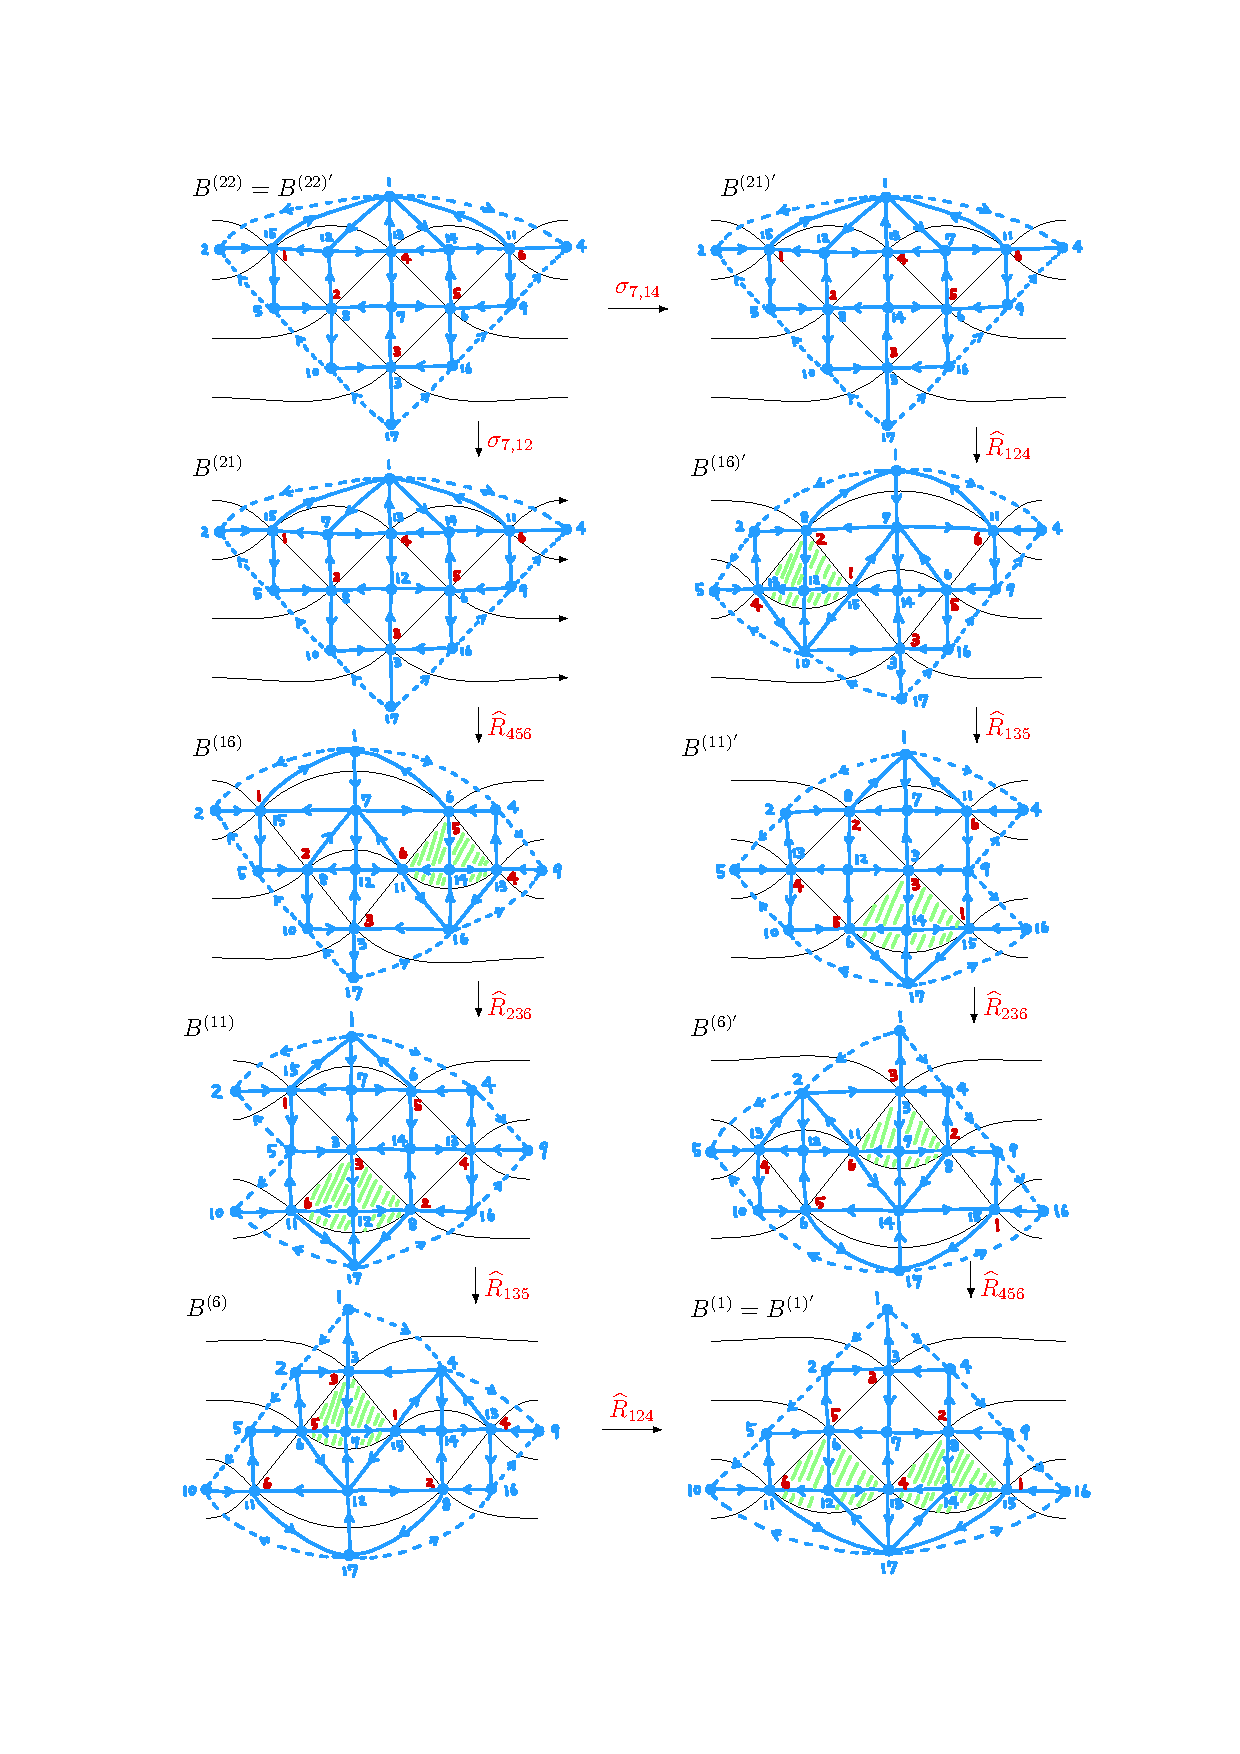
\includegraphics[clip,scale=0.77]{../assets/1053/tetra-butterfly.pdf}
\vspace{-2mm}
\caption{Cluster transformations $\widehat{R}_{ijk}$.
The wiring diagrams have 6 crossings (red).
The quivers (blue) have 17 vertices.
Triangles relevant to the image of $\hat{R}_{ijk}$ are hatched in green.
The seeds \smash{$\bigl(B^{(t)}, \bY^{(t)}\bigr)$} and~\smash{$\bigl(B^{(t)\prime}, \bY^{(t)\prime}\bigr)$} will be
explained in detail in Section \ref{ss:ms}.}\label{fig:bTE}\vspace{-1mm}
\end{figure}


\subsection{Monomial solutions to the tetrahedron equation}\label{ss:ms}

In this subsection, we provide additional details regarding Figure~\ref{fig:bTE} and Proposition~\ref{pr:sy}. Let
\smash{$\bigl(B^{(1)}, \bY^{(1)}\bigr) = \bigl(B^{(1)\prime}, \bY^{(1)\prime}\bigr)$} be the
initial quantum $y$-seed corresponding to the quiver at the bottom of
Figure~\ref{fig:bTE}. The quantum $y$-seeds $\bigl(B^{(t)}, \bY^{(t)}\bigr)$
and $\bigl(B^{(t)\prime}, \bY^{(t)\prime}\bigr)$ ($t=2, \dots, 21$), which
pertain to the left and the right paths are determined from it by the
mutation sequences, and we have just shown that the final results
coincide, i.e.,
$\bigl(B^{(22)}, \bY^{(22)}\bigr) = \bigl(B^{(22)\prime}, \bY^{(22)\prime}\bigr)$. Set~\smash{$\bY^{(t)}=\bigl(Y^{(t)}_1,\dotsc, Y^{(t)}_{17}\bigr)$} and
\smash{$\bY^{(t)\prime}=\bigl(Y^{(t)\prime}_1,\dotsc, Y^{(t)\prime}_{17}\bigr)$}.

The quantum $y$-seeds $\bigl(B^{(t)}, \bY^{(t)}\bigr)$ ($t=2,\dotsc, 21$) are
determined from the initial one $\bigl(B^{(1)},\allowbreak \bY^{(1)}\bigr) $ by
\begin{gather}
\bigl(B^{(1)}, \bY^{(1)}\bigr) \underset{\varepsilon_1}{\overset{\mu_{14}}{\longleftrightarrow}}
\bigl(B^{(2)}, \bY^{(2)}\bigr) \underset{\varepsilon_2}{\overset{\mu_{13}}{\longleftrightarrow}}
\bigl(B^{(3)}, \bY^{(3)}\bigr) \underset{\varepsilon_3}{\overset{\mu_{15}}{\longleftrightarrow}}
\bigl(B^{(4)}, \bY^{(4)}\bigr)\nonumber
\\
\phantom{\bigl(B^{(1)}, \bY^{(1)}\bigr)}{}
 \underset{\varepsilon_4}{\overset{\mu_{8}}{\longleftrightarrow}}
\bigl(B^{(5)}, \bY^{(5)}\bigr) \overset{\sigma_{13,15}\sigma_{8,14}}{\longleftrightarrow}
\bigl(B^{(6)}, \bY^{(6)}\bigr),\nonumber
\\
\bigl(B^{(6)}, \bY^{(6)}\bigr) \underset{\varepsilon_1}{\overset{\mu_{7}}{\longleftrightarrow}}
\bigl(B^{(7)}, \bY^{(7)}\bigr) \underset{\varepsilon_2}{\overset{\mu_{6}}{\longleftrightarrow}}
\bigl(B^{(8)}, \bY^{(8)}\bigr) \underset{\varepsilon_3}{\overset{\mu_{15}}{\longleftrightarrow}}
\bigl(B^{(9)}, \bY^{(9)}\bigr)\nonumber
\\
\phantom{\bigl(B^{(6)}, \bY^{(6)}\bigr)}{}
\underset{\varepsilon_4}{\overset{\mu_{3}}{\longleftrightarrow} }
\bigl(B^{(10)}, \bY^{(10)}\bigr) \overset{\sigma_{6,15}\sigma_{3,7}}{\longleftrightarrow}
\bigl(B^{(11)}, \bY^{(11)}\bigr),\nonumber
\\
\bigl(B^{(11)}, \bY^{(11)}\bigr) \underset{\varepsilon_1}{\overset{\mu_{12}}{\longleftrightarrow} }
\bigl(B^{(12)}, \bY^{(12)}\bigr) \underset{\varepsilon_2}{\overset{\mu_{11}}{\longleftrightarrow} }
\bigl(B^{(13)}, \bY^{(13)}\bigr) \underset{\varepsilon_3}{\overset{\begin{color}{red}\mu_{8}\end{color}}{\longleftrightarrow} }
\bigl(B^{(14)}, \bY^{(14)}\bigr)\nonumber
\\
\phantom{\bigl(B^{(11)}, \bY^{(11)}\bigr)}{}
 \underset{\varepsilon_4}{ \overset{\mu_{3}}{\longleftrightarrow}}
\bigl(B^{(15)}, \bY^{(15)}\bigr) \overset{\sigma_{8,11}\sigma_{3,12}}{\longleftrightarrow}
\bigl(B^{(16)}, \bY^{(16)}\bigr),\nonumber
\\
\bigl(B^{(16)}, \bY^{(16)}\bigr) \underset{\varepsilon_1}{\overset{\begin{color}{red}\mu_{14}\end{color}}{\longleftrightarrow}}
\bigl(B^{(17)}, \bY^{(17)}\bigr) \underset{\varepsilon_2}{\overset{\mu_{11}}{\longleftrightarrow}}
\bigl(B^{(18)}, \bY^{(18)}\bigr) \underset{\varepsilon_3}{\overset{\mu_{13}}{\longleftrightarrow}}
\bigl(B^{(19)}, \bY^{(19)}\bigr)\nonumber
\\
\phantom{\bigl(B^{(16)}, \bY^{(16)}\bigr) }{}
\underset{\varepsilon_4}{ \overset{\mu_{6}}{\longleftrightarrow}}
\bigl(B^{(20)}, \bY^{(20)}\bigr) \overset{\sigma_{11,13}\sigma_{6,14}}{\longleftrightarrow}
\bigl(B^{(21)}, \bY^{(21)}\bigr),\nonumber
\\
\bigl(B^{(21)}, \bY^{(21)}\bigr) \overset{\sigma_{7,12}}{\longleftrightarrow}
\bigl(B^{(22)}, \bY^{(22)}\bigr),\label{b21L}
\end{gather}
where the notation is parallel with \eqref{mus}. In particular the
choice of signs $\varepsilon_1, \dots, \varepsilon_4$ does not
influence the mutations themselves.
%
According to \eqref{rhat}, each line in the above corresponds to a~cluster transformation appearing in the left path of
Figure \ref{fig:bTE} as follows:
\begin{gather}
\widehat{R}_{124} =
\mathrm{Ad}\bigl(\Psi_q\bigl(\bigl(Y^{(1)}_{14}\bigr)^{\varepsilon_1}\bigr)^{\varepsilon_1}\bigr)\tau_{14,\varepsilon_1}
\mathrm{Ad}\bigl(\Psi_q\bigl(\bigl(Y^{(2)}_{13}\bigr)^{\varepsilon_2}\bigr)^{\varepsilon_2}\bigr)\tau_{13,\varepsilon_2}\nonumber
\\
\phantom{\widehat{R}_{124} =}{} \times
\mathrm{Ad}\bigl(\Psi_q\bigl(\bigl(Y^{(3)}_{15}\bigr)^{\varepsilon_3}\bigr)^{\varepsilon_3}\bigr)\tau_{15,\varepsilon_3}
\mathrm{Ad}\bigl(\Psi_q\bigl(\bigl(Y^{(4)}_{8}\bigr)^{\varepsilon_4}\bigr)^{\varepsilon_4}\bigr)\tau_{8,\varepsilon_4}
\sigma_{13,15}\sigma_{8,14},\nonumber
\\
\widehat{R}_{135} =
\mathrm{Ad}\bigl(\Psi_q\bigl(\bigl(Y^{(6)}_{7}\bigr)^{\varepsilon_1}\bigr)^{\varepsilon_1}\bigr)\tau_{7,\varepsilon_1}
\mathrm{Ad}\bigl(\Psi_q\bigl(\bigl(Y^{(7)}_{6}\bigr)^{\varepsilon_2}\bigr)^{\varepsilon_2}\bigr)\tau_{6,\varepsilon_2}\nonumber
\\
\phantom{\widehat{R}_{135} =}{} \times
\mathrm{Ad}\bigl(\Psi_q\bigl(\bigl(Y^{(8)}_{15}\bigr)^{\varepsilon_3}\bigr)^{\varepsilon_3}\bigr)\tau_{15,\varepsilon_3}
\mathrm{Ad}\bigl(\Psi_q\bigl(\bigl(Y^{(9)}_{3}\bigr)^{\varepsilon_4}\bigr)^{\varepsilon_4}\bigr)\tau_{3,\varepsilon_4}
\sigma_{6,15}\sigma_{3,7},\nonumber
\\
\widehat{R}_{236} =
\mathrm{Ad}\bigl(\Psi_q\bigl(\bigl(Y^{(11)}_{12}\bigr)^{\varepsilon_1}\bigr)^{\varepsilon_1}\bigr)\tau_{12,\varepsilon_1}
\mathrm{Ad}\bigl(\Psi_q\bigl(\bigl(Y^{(12)}_{11}\bigr)^{\varepsilon_2}\bigr)^{\varepsilon_2}\bigr)\tau_{11,\varepsilon_2}\nonumber
\\
\phantom{\widehat{R}_{236} =}{} \times
\mathrm{Ad}\bigl(\Psi_q\bigl(\bigl(Y^{(13)}_{8}\bigr)^{\varepsilon_3}\bigr)^{\varepsilon_3}\bigr)\tau_{8,\varepsilon_3}
\mathrm{Ad}\bigl(\Psi_q\bigl(\bigl(Y^{(14)}_{3}\bigr)^{\varepsilon_4}\bigr)^{\varepsilon_4}\bigr)\tau_{3,\varepsilon_4}
\sigma_{8,11}\sigma_{3,12},\nonumber
\\
\widehat{R}_{456} =
\mathrm{Ad}\bigl(\Psi_q\bigl(\bigl(Y^{(16)}_{14}\bigr)^{\varepsilon_1}\bigr)^{\varepsilon_1}\bigr)\tau_{14,\varepsilon_1}
\mathrm{Ad}\bigl(\Psi_q\bigl(\bigl(Y^{(17)}_{11}\bigr)^{\varepsilon_2}\bigr)^{\varepsilon_2}\bigr)\tau_{11,\varepsilon_2}\nonumber
\\
\phantom{\widehat{R}_{456} =}{} \times
\mathrm{Ad}\bigl(\Psi_q\bigl(\bigl(Y^{(18)}_{13}\bigr)^{\varepsilon_3}\bigr)^{\varepsilon_3}\bigr)\tau_{13,\varepsilon_3}
\mathrm{Ad}\bigl(\Psi_q\bigl(\bigl(Y^{(19)}_{6}\bigr)^{\varepsilon_4}\bigr)^{\varepsilon_4}\bigr)\tau_{6,\varepsilon_4}
\sigma_{11,13}\sigma_{6,14}.\label{r124a}
\end{gather}

The quantum $y$-seeds $\bigl(B^{(t)\prime}, Y^{(t)\prime}\bigr)$
($t=2, \dots, 21$) are determined from the initial one
$\bigl(B^{(1)\prime},\allowbreak Y^{(1)\prime}\bigr)$ by
\begin{gather}
\bigl(B^{(1)\prime}, \bY^{(1)\prime}\bigr) \underset{\varepsilon_1}{\overset{\mu_{12}}{\longleftrightarrow}}
\bigl(B^{(2)\prime}, \bY^{(2)\prime}\bigr) \underset{\varepsilon_2}{\overset{\mu_{11}}{\longleftrightarrow}}
\bigl(B^{(3)\prime}, \bY^{(3)\prime}\bigr) \underset{\varepsilon_3}{\overset{\mu_{13}}{\longleftrightarrow}}
\bigl(B^{(4)\prime}, \bY^{(4)\prime}\bigr)\nonumber
\\
\phantom{\bigl(B^{(1)\prime}, \bY^{(1)\prime}\bigr) }{}
\underset{\varepsilon_4}{\overset{\mu_{6}}{\longleftrightarrow}}
\bigl(B^{(5)\prime}, \bY^{(5)\prime}\bigr) \overset{\sigma_{11,13}\sigma_{6,12}}{\longleftrightarrow}
\bigl(B^{(6)\prime}, \bY^{(6)\prime}\bigr),\nonumber
\\
\bigl(B^{(6)\prime}, \bY^{(6)\prime}\bigr) \underset{\varepsilon_1}{\overset{\mu_{7}}{\longleftrightarrow}}
\bigl(B^{(7)\prime}, \bY^{(7)\prime}\bigr) \underset{\varepsilon_2}{\overset{\mu_{11}}{\longleftrightarrow}}
\bigl(B^{(8)\prime}, \bY^{(8)\prime}\bigr) \underset{\varepsilon_3}{\overset{\mu_{8}}{\longleftrightarrow}}
\bigl(B^{(9)\prime}, \bY^{(9)\prime}\bigr)\nonumber
\\
\phantom{\bigl(B^{(6)\prime}, \bY^{(6)\prime}\bigr)}{}
\underset{\varepsilon_4}{\overset{\mu_{3}}{\longleftrightarrow}}
\bigl(B^{(10)\prime}, \bY^{(10)\prime}\bigr) \overset{\sigma_{8,11}\sigma_{3,7}}{\longleftrightarrow}
\bigl(B^{(11)\prime}, \bY^{(11)\prime}\bigr),\nonumber
\\
\bigl(B^{(11)\prime}, \bY^{(11)\prime}\bigr) \underset{\varepsilon_1}{\overset{\mu_{14}}{\longleftrightarrow}}
\bigl(B^{(12)\prime}, \bY^{(12)\prime}\bigr) \underset{\varepsilon_2}{\overset{\begin{color}{red}\mu_{6}\end{color}}{\longleftrightarrow}}
\bigl(B^{(13)\prime}, \bY^{(13)\prime}\bigr) \underset{\varepsilon_3}{\overset{\mu_{15}}{\longleftrightarrow}}
\bigl(B^{(14)\prime}, \bY^{(14)\prime}\bigr)\nonumber
\\
\phantom{\bigl(B^{(11)\prime}, \bY^{(11)\prime}\bigr)}{}
\underset{\varepsilon_4}{\overset{\mu_{3}}{\longleftrightarrow}}
\bigl(B^{(15)\prime}, \bY^{(15)\prime}\bigr) \overset{\sigma_{6,15}\sigma_{3,14}}{\longleftrightarrow}
\bigl(B^{(16)\prime}, \bY^{(16)\prime}\bigr)\nonumber
\\
\bigl(B^{(16)\prime}, \bY^{(16)\prime}\bigr) \underset{\varepsilon_1}{\overset{\begin{color}{red}\mu_{12}\end{color}}{\longleftrightarrow} }
\bigl(B^{(17)\prime}, \bY^{(17)\prime}\bigr) \underset{\varepsilon_2}{\overset{\mu_{13}}{\longleftrightarrow} }
\bigl(B^{(18)\prime}, \bY^{(18)\prime}\bigr) \underset{\varepsilon_3}{\overset{\mu_{15}}{\longleftrightarrow} }
\bigl(B^{(19)\prime}, \bY^{(19)\prime}\bigr)\nonumber
\\
\phantom{\bigl(B^{(16)\prime}, \bY^{(16)\prime}\bigr)}{}
\underset{\varepsilon_4}{\overset{\mu_{8}}{\longleftrightarrow} }
\bigl(B^{(20)\prime}, \bY^{(20)\prime}\bigr) \overset{\sigma_{13,15}\sigma_{8,12}}{\longleftrightarrow}
\bigl(B^{(21)\prime}, \bY^{(21)\prime}\bigr),\nonumber
\\
\bigl(B^{(21)\prime}, \bY^{(21)\prime}\bigr) \overset{\sigma_{7,14}}{\longleftrightarrow}
\bigl(B^{(22)\prime}, \bY^{(22)\prime}\bigr).\label{b11R}
\end{gather}
They correspond to the cluster transformations in the right path of Figure \ref{fig:bTE} as follows:
\begin{align}
\widehat{R}_{456} ={}&
\mathrm{Ad}\bigl(\Psi_q\bigl(\bigl(Y^{(1)\prime}_{12}\bigr)^{\varepsilon_1}\bigr)^{\varepsilon_1}\bigr)\tau_{12,\varepsilon_1}
\mathrm{Ad}\bigl(\Psi_q\bigl(\bigl(Y^{(2)\prime}_{11}\bigr)^{\varepsilon_2}\bigr)^{\varepsilon_2}\bigr)\tau_{11,\varepsilon_2}\nonumber
\\
& \times
\mathrm{Ad}\bigl(\Psi_q\bigl(\bigl(Y^{(3)\prime}_{13}\bigr)^{\varepsilon_3}\bigr)^{\varepsilon_z3}\bigr)\tau_{13,\varepsilon_3}
\mathrm{Ad}\bigl(\Psi_q\bigl(\bigl(Y^{(4)\prime}_{6}\bigr)^{\varepsilon_4}\bigr)^{\varepsilon_4}\bigr)\tau_{6,\varepsilon_4}
\sigma_{11,13}\sigma_{6,12},\nonumber
\\
\widehat{R}_{236} ={}&
\mathrm{Ad}\bigl(\Psi_q\bigl(\bigl(Y^{(6)\prime}_{7}\bigr)^{\varepsilon_1}\bigr)^{\varepsilon_1}\bigr)\tau_{7,\varepsilon_1}
\mathrm{Ad}\bigl(\Psi_q\bigl(\bigl(Y^{(7)\prime}_{11}\bigr)^{\varepsilon_2}\bigr)^{\varepsilon_2}\bigr)\tau_{11,\varepsilon_2}\nonumber
\\
& \times
\mathrm{Ad}\bigl(\Psi_q\bigl(\bigl(Y^{(8)\prime}_{8}\bigr)^{\varepsilon_3}\bigr)^{\varepsilon_3}\bigr)\tau_{8,\varepsilon_3}
\mathrm{Ad}\bigl(\Psi_q\bigl(\bigl(Y^{(9)\prime}_{3}\bigr)^{\varepsilon_4}\bigr)^{\varepsilon_4}\bigr)\tau_{3,\varepsilon_4}
\sigma_{8,11}\sigma_{3,7},\nonumber
\\
\widehat{R}_{135} ={}&
\mathrm{Ad}\bigl(\Psi_q\bigl(\bigl(Y^{(11)\prime}_{14}\bigr)^{\varepsilon_1}\bigr)^{\varepsilon_1}\bigr)\tau_{14,\varepsilon_1}
\mathrm{Ad}\bigl(\Psi_q\bigl(\bigl(Y^{(12)\prime}_{6}\bigr)^{\varepsilon_2}\bigr)^{\varepsilon_2}\bigr)\tau_{6,\varepsilon_2}\nonumber
\\
& \times
\mathrm{Ad}\bigl(\Psi_q\bigl(\bigl(Y^{(13)\prime}_{15}\bigr)^{\varepsilon_3}\bigr)^{\varepsilon_3}\bigr)\tau_{15,\varepsilon_3}
\mathrm{Ad}\bigl(\Psi_q\bigl(\bigl(Y^{(14)\prime}_{3}\bigr)^{\varepsilon_4}\bigr)^{\varepsilon_4}\bigr)\tau_{3,\varepsilon_4}
\sigma_{6,15}\sigma_{3,14},\nonumber
\\
\widehat{R}_{124} ={}&
\mathrm{Ad}\bigl(\Psi_q\bigl(\bigl(Y^{(16)\prime}_{12}\bigr)^{\varepsilon_1}\bigr)^{\varepsilon_1}\bigr)\tau_{12,\varepsilon_1}
\mathrm{Ad}\bigl(\Psi_q\bigl(\bigl(Y^{(17)\prime}_{13}\bigr)^{\varepsilon_2}\bigr)^{\varepsilon_2}\bigr)\tau_{13,\varepsilon_2}\nonumber
\\
& \times
\mathrm{Ad}\bigl(\Psi_q\bigl(\bigl(Y^{(18)\prime}_{15}\bigr)^{\varepsilon_3}\bigr)^{\varepsilon_3}\bigr)\tau_{15,\varepsilon_3}
\mathrm{Ad}\bigl(\Psi_q\bigl(\bigl(Y^{(19)\prime}_{8}\bigr)^{\varepsilon_4}\bigr)^{\varepsilon_4}\bigr)\tau_{8,\varepsilon_4}
\sigma_{13,15}\sigma_{8,12}.\label{r456b}
\end{align}
Although the formulas \eqref{r124a} and \eqref{r456b} may appear distinct,
they all signify the same transformation described in Proposition \ref{pr:RY}
for the corresponding subsets of $Y$-variables.
This fact justifies denoting them by the common symbol $\widehat{R}$.

\begin{Remark}\label{re:red}
 Consider the tropical $y$-seeds generated by the same mutation
 sequences from the initial one
 \smash{$\bigl(B^{(1)}, y^{(1)}\bigr) = \bigl(B^{(1)\prime}, y^{(1)\prime}\bigr)$}. Suppose
 \smash{$y^{(1)}_i = y^{(1)\prime}_i$} is positive for all $i=1, \dots,
 17$. Then the four mutations highlighted in red in \eqref{b21L}
 and \eqref{b11R} are associated to a negative tropical sign of the
 $y$-variable at the mutation point (the $y$-seed in the left), while
 the remaining ones are positive.
\end{Remark}

Let us introduce the monomial parts of the cluster transformations \eqref{r124a} and \eqref{r456b}
\begin{gather*}
\tau_{124 | \varepsilon_1,\varepsilon_2,\varepsilon_3,\varepsilon_4} :=
\tau_{14,\varepsilon_1}\tau_{13,\varepsilon_2}\tau_{15,\varepsilon_3}\tau_{8,\varepsilon_4}\sigma_{13,15}\sigma_{8,14}\colon\
 \mathcal{Y}\bigl(B^{(6)}\bigr) \rightarrow \mathcal{Y}\bigl(B^{(1)}\bigr),
\\
\tau_{135 | \varepsilon_1,\varepsilon_2,\varepsilon_3,\varepsilon_4} :=
\tau_{7,\varepsilon_1}\tau_{6,\varepsilon_2}\tau_{15,\varepsilon_3}\tau_{3,\varepsilon_4}\sigma_{6,15}\sigma_{3,7}\colon\
 \mathcal{Y}\bigl(B^{(11)}\bigr) \rightarrow \mathcal{Y}\bigl(B^{(6)}\bigr),
\\
\tau_{236 | \varepsilon_1,\varepsilon_2,\varepsilon_3,\varepsilon_4} :=
\tau_{12,\varepsilon_1}\tau_{11,\varepsilon_2}\tau_{8,\varepsilon_3}\tau_{3,\varepsilon_4}\sigma_{8,11}\sigma_{3,12}\colon\
 \mathcal{Y}\bigl(B^{(16)}\bigr) \rightarrow \mathcal{Y}\bigl(B^{(11)}\bigr),
\\
\tau_{456 | \varepsilon_1,\varepsilon_2,\varepsilon_3,\varepsilon_4} :=
\tau_{14,\varepsilon_1}\tau_{11,\varepsilon_2}\tau_{13,\varepsilon_3}\tau_{6,\varepsilon_4}\sigma_{11,13}\sigma_{6,14}\colon\
 \mathcal{Y}\bigl(B^{(21)}\bigr) \rightarrow \mathcal{Y}\bigl(B^{(16)}\bigr),
\\
\tau'_{456 | \varepsilon_1,\varepsilon_2,\varepsilon_3,\varepsilon_4} :=
\tau_{12,\varepsilon_1}\tau_{11,\varepsilon_2}\tau_{13,\varepsilon_3}\tau_{6,\varepsilon_4}\sigma_{11,13}\sigma_{6,12}\colon\
 \mathcal{Y}\bigl(B^{(6)\prime}\bigr) \rightarrow \mathcal{Y}\bigl(B^{(1)\prime}\bigr),
\\
\tau'_{236 | \varepsilon_1,\varepsilon_2,\varepsilon_3,\varepsilon_4} :=
\tau_{7,\varepsilon_1}\tau_{11,\varepsilon_2}\tau_{8,\varepsilon_3}\tau_{3,\varepsilon_4}\sigma_{8,11}\sigma_{3,7}\colon\
 \mathcal{Y}\bigl(B^{(11)\prime}\bigr) \rightarrow \mathcal{Y}\bigl(B^{(6)\prime}\bigr),
\\
\tau'_{135 | \varepsilon_1,\varepsilon_2,\varepsilon_3,\varepsilon_4} :=
\tau_{14,\varepsilon_1}\tau_{6,\varepsilon_2}\tau_{15,\varepsilon_3}\tau_{3,\varepsilon_4}\sigma_{6,15}\sigma_{3,14}\colon\
 \mathcal{Y}\bigl(B^{(16)\prime}\bigr) \rightarrow \mathcal{Y}\bigl(B^{(11)\prime}\bigr),
\\
\tau'_{124 | \varepsilon_1,\varepsilon_2,\varepsilon_3,\varepsilon_4} :=
\tau_{12,\varepsilon_1}\tau_{13,\varepsilon_2}\tau_{15,\varepsilon_3}\tau_{8,\varepsilon_4}\sigma_{13,15}\sigma_{8,12}\colon\
 \mathcal{Y}\bigl(B^{(21)\prime}\bigr) \rightarrow \mathcal{Y}\bigl(B^{(16)\prime}\bigr).
\end{gather*}
The primes in $\tau'_{\!ijk | \varepsilon_1,\varepsilon_2,\varepsilon_3,\varepsilon_4}$
are added just for distinction.
The maps $\tau_{\!ijk | \varepsilon_1,\varepsilon_2,\varepsilon_3,\varepsilon_4}$ and
$\tau'_{\!ijk | \varepsilon_1,\varepsilon_2,\varepsilon_3,\varepsilon_4}$
consistently adhere to $\tau_{\varepsilon_1,\varepsilon_2,\varepsilon_3,\varepsilon_4}$ in
\eqref{taue} with respect to the subset of $Y$-variables.

Now we are ready to explain monomial solutions to the twisted tetrahedron equation.
Proposition \ref{pr:sy}, Figure \ref{fig:bTE} and Remark \ref{re:sgni} indicate
the equality of the tropical $y$-variables $y^{(22)} = y^{(22)\prime}$ {\em provided} that
all the signs associated with the monomial part of the mutation are chosen to be the tropical signs.
Considering Remark \ref{re:red} alongside, we find that
\begin{gather}
\tau_{124| + + + +} \tau_{135| + + + +}\tau_{236| + + - +}\tau_{456| - + + +}\sigma_{7,12}\nonumber\\
\qquad
=
\tau'_{456| + + + +}\tau'_{236| + + + +}\tau'_{135| + - + +}\tau'_{124| - + + +}\sigma_{7,14}\label{ihte}
\end{gather}
is valid instead of the naive choice of $\tau_{ijk| ++++}$ and $\tau'_{ijk| ++++}$ everywhere.
This is an inhomogeneous version of the twisted tetrahedron equation,
as the maps involved are not always uniform in their sign indices.
%
The coincident image of \smash{$Y^{(22)}_1, \dots, Y^{(22)}_{17}$} by the
two sides are sign coherent monomials in the initial $Y$-variables
$\bY^{(1)} = (Y_1,\dotsc, Y_{17})$. Their explicit form is available
in~\eqref{y22}.

A natural question is whether there are monomial solutions to the twisted tetrahedron equation
with the signs homogeneously chosen as $(\varepsilon_1,\varepsilon_2,\varepsilon_3,\varepsilon_4)$
\begin{gather}
\tau_{124| \varepsilon_1,\varepsilon_2,\varepsilon_3,\varepsilon_4}
\tau_{135| \varepsilon_1,\varepsilon_2,\varepsilon_3,\varepsilon_4}
\tau_{236| \varepsilon_1,\varepsilon_2,\varepsilon_3,\varepsilon_4}
\tau_{456| \varepsilon_1,\varepsilon_2,\varepsilon_3,\varepsilon_4} \sigma_{7,12}\nonumber
\\
\qquad=
\tau'_{456| \varepsilon_1,\varepsilon_2,\varepsilon_3,\varepsilon_4}
\tau'_{236| \varepsilon_1,\varepsilon_2,\varepsilon_3,\varepsilon_4}
\tau'_{135| \varepsilon_1,\varepsilon_2,\varepsilon_3,\varepsilon_4}
\tau'_{124| \varepsilon_1,\varepsilon_2,\varepsilon_3,\varepsilon_4}\sigma_{7,14}.\label{hteq}
\end{gather}
The answer is given by a direct calculation as follows.
\begin{Proposition} \label{pr:mono}
The monomial part
satisfies the tetrahedron equation \eqref{hteq}
if and only if~${\varepsilon_1=-\varepsilon_4 = -}$, i.e.,
$(\varepsilon_1,\varepsilon_2,\varepsilon_3,\varepsilon_4) \in
\{(-,+,+,+), (-,+,-,+), (-,-,+,+), (-,-,-,+)\}$.
\end{Proposition}
Examples \ref{ex:1} and \ref{ex:2} describe the monomial parts
$\tau_{--++}$ and $\tau_{-+-+}$ explicitly.
Analogous information is supplied for the remaining two cases in Appendix \ref{ap:sup}.

\subsection{Dilogarithm identities}\label{ss:did}

Now we turn to the dilogarithm identities that will be utilized later.
Substitute \eqref{r124a} and \eqref{r456b} into the
left-hand side and the right-hand side of \eqref{TE1} respectively.
The result takes the form
\begin{gather}
\mathrm{Ad}\bigl(
\Psi_q(U_1)^{\varepsilon_1} \dotsm \Psi_q(U_4)^{\varepsilon_4}\bigr)
\tau_{124| \varepsilon_1, \varepsilon_2, \varepsilon_3, \varepsilon_4}
\mathrm{Ad}\bigl(
\Psi_q(U_5)^{\varepsilon_1} \dotsm \Psi_q(U_8)^{\varepsilon_4}\bigr)
\tau_{135| \varepsilon_1, \varepsilon_2, \varepsilon_3, \varepsilon_4}\nonumber
\\
\phantom{\qquad =}{}\times
\mathrm{Ad}\bigl(
\Psi_q(U_9)^{\varepsilon_1} \dotsm \Psi_q(U_{12})^{\varepsilon_4}\bigr)
\tau_{236 | \varepsilon_1, \varepsilon_2, \varepsilon_3, \varepsilon_4}\nonumber
\\
\phantom{\qquad =}{}\times
\mathrm{Ad}\bigl(
\Psi_q(U_{13})^{\varepsilon_1} \dotsm \Psi_q(U_{16})^{\varepsilon_4}\bigr)
\tau_{456| \varepsilon_1, \varepsilon_2, \varepsilon_3, \varepsilon_4}\sigma_{7,12}\nonumber
\\
\qquad {}=
\mathrm{Ad}\bigl(
\Psi_q\bigl(U'_1\bigr)^{\varepsilon_1} \dotsm \Psi_q\bigl(U'_4\bigr)^{\varepsilon_4}\bigr)
\tau'_{456| \varepsilon_1, \varepsilon_2, \varepsilon_3, \varepsilon_4}
\mathrm{Ad}\bigl(
\Psi_q\bigl(U'_5\bigr)^{\varepsilon_1} \dotsm \Psi_q\bigl(U'_8\bigr)^{\varepsilon_4}\bigr)
\tau'_{236| \varepsilon_1, \varepsilon_2, \varepsilon_3, \varepsilon_4}\nonumber
\\
\phantom{\qquad =}{} \times
\mathrm{Ad}\bigl(
\Psi_q\bigl(U'_9\bigr)^{\varepsilon_1} \dotsm \Psi_q\bigl(U'_{12}\bigr)^{\varepsilon_4}\bigr)
\tau'_{135| \varepsilon_1, \varepsilon_2, \varepsilon_3, \varepsilon_4}\nonumber
\\
\phantom{\qquad =}{} \times
\mathrm{Ad}\bigl(
\Psi_q\bigl(U'_{13}\bigr)^{\varepsilon_1} \dotsm \Psi_q\bigl(U'_{16}\bigr)^{\varepsilon_4}\bigr)
\tau'_{124| \varepsilon_1, \varepsilon_2, \varepsilon_3, \varepsilon_4}\sigma_{7,14},\label{psiu}
\end{gather}
where $U_t$ and $U'_t$ ($t=1, \dots, 16$) denote the $Y$-variables
depending on
$(\varepsilon_1, \varepsilon_2, \varepsilon_3, \varepsilon_4)$.
%
Pushing the monomial parts to the right brings \eqref{psiu} into the form
\begin{gather}
\mathrm{Ad}\bigl(\Psi_q(Z_1)^{\varepsilon_1}\dotsm \Psi_q(Z_{16})^{\varepsilon_{4}}\bigr)
\tau_{124|\varepsilon_1,\varepsilon_2,\varepsilon_3,\varepsilon_4}
\tau_{135|\varepsilon_1,\varepsilon_2,\varepsilon_3,\varepsilon_4}
\tau_{236|\varepsilon_1,\varepsilon_2,\varepsilon_3,\varepsilon_4}
\tau_{456|\varepsilon_1,\varepsilon_2,\varepsilon_3,\varepsilon_4}\sigma_{7,12}\nonumber
\\
\qquad=
\mathrm{Ad}\bigl(\Psi_q\bigl(Z'_1\bigr)^{\varepsilon_1}\dotsm \Psi_q\bigl(Z'_{16}\bigr)^{\varepsilon_{4}}\bigr)
\tau'_{456|\varepsilon_1,\varepsilon_2,\varepsilon_3,\varepsilon_4}
\tau'_{236|\varepsilon_1,\varepsilon_2,\varepsilon_3,\varepsilon_4}\nonumber
\\
\phantom{\qquad=}{}\times
\tau'_{135|\varepsilon_1,\varepsilon_2,\varepsilon_3,\varepsilon_4}
\tau'_{124|\varepsilon_1,\varepsilon_2,\varepsilon_3,\varepsilon_4}\sigma_{7,14},\label{zteq}
\end{gather}
where $Z_i$ and $Z'_i$ are monomials of $Y_1, \dots, Y_{16}$
determined by
\begin{align}\label{zu}
Z_i = \begin{cases} U_i, & i = 1,\dotsc, 4,
\\
 \tau_{124|\varepsilon_1,\varepsilon_2,\varepsilon_3,\varepsilon_4}
 (U_i), & i=5,\dotsc, 8,
\\
\tau_{124|\varepsilon_1,\varepsilon_2,\varepsilon_3,\varepsilon_4}
\tau_{135|\varepsilon_1,\varepsilon_2,\varepsilon_3,\varepsilon_4}
(U_i), & i=9, \ldots, 12,
\\
\tau_{124|\varepsilon_1,\varepsilon_2,\varepsilon_3,\varepsilon_4}
\tau_{135|\varepsilon_1,\varepsilon_2,\varepsilon_3,\varepsilon_4}
\tau_{236|\varepsilon_1,\varepsilon_2,\varepsilon_3,\varepsilon_4}
(U_i), & i=13, \ldots, 16.
\end{cases}
\end{align}
The elements $Z'_i$ are similarly determined from the
right-hand side of \eqref{psiu}.
%
From \eqref{zteq} and Proposition~\ref{pr:mono}, we deduce
\begin{align}\label{adeq}
\mathrm{Ad}\bigl(\Psi_q(Z_1)^{\varepsilon_1}\cdots \Psi_q(Z_{16})^{\varepsilon_{4}}\bigr)
=\mathrm{Ad}\bigl(\Psi_q\bigl(Z'_1\bigr)^{\varepsilon_1}\cdots \Psi_q\bigl(Z'_{16}\bigr)^{\varepsilon_{4}}\bigr)
\end{align}
for $(\varepsilon_1,\varepsilon_2,\varepsilon_3,\varepsilon_4) \in
\{(-,+,+,+), (-,+,-,+), (-,-,+,+), (-,-,-,+)\}$.
Actually a stronger equality holds.

\begin{Proposition}\label{pr:dilog}
For $(\varepsilon_1,\varepsilon_2,\varepsilon_3,\varepsilon_4) \in \{(-,+,-,+), (-,-,+,+)\}$,
the products of quantum dilogarithms within $\mathrm{Ad}$ in \eqref{adeq}
are well defined formal Laurent series in
the nine $Y$-variables
$Y_3$, $Y_6$, $Y_7$, $Y_8$, $Y_{11}$, $Y_{12}$, $Y_{13}$, $Y_{14}$ and $Y_{15}$.
Moreover, they are equal, i.e.,
\begin{align}\label{pseq}
\Psi_q(Z_1)^{\varepsilon_1}\dotsm \Psi_q(Z_{16})^{\varepsilon_{4}}
=
\Psi_q\bigl(Z'_1\bigr)^{\varepsilon_1}\dotsm \Psi_q\bigl(Z'_{16}\bigr)^{\varepsilon_{4}}.
\end{align}
\end{Proposition}

\begin{proof}
 We show the claim for
 $(\varepsilon_1,\varepsilon_2,\varepsilon_3,\varepsilon_4)
 =(-,-,+,+)$. The case $(-,+,-,+)$ is similar. The data $Z_1,
 \dots, Z_{16}$ for
 $(\varepsilon_1,\varepsilon_2,\varepsilon_3,\varepsilon_4)=(-,-,+,+)$
 is given by
\begin{align}\label{zdL}
\begin{pmatrix}
Y_{14}^{-1} &
qY^{-1}_{13}Y^{-1}_{14} &
q^{-1}Y_{14}Y_{15} &
q^{-2}Y_{8}Y_{14}Y_{15}
\\
q^{2}Y^{-1}_7Y^{-1}_{13}Y^{-1}_{14} &
q^3Y^{-1}_6Y^{-1}_7Y^{-1}_{13}Y^{-1}_{14} &
q^{-3}Y_7Y_8Y_{14}Y_{15} &
q^{-4}Y_3Y_7Y_8Y_{14}Y_{15}
\\
Y^{-1}_{12} &
qY^{-1}_{11}Y^{-1}_{12} &
q^{-1}Y_{12}Y_{13}&
q^{-2}Y_6Y_{12} Y_{13}
\\
Y^{-1}_{7} &
qY^{-1}_6Y^{-1}_7 &
q^{-1}Y_7Y_8 &
q^{-2}Y_3Y_7Y_8
\end{pmatrix},
\end{align}
where the element at $i$th row and the $j$th column from the top left signifies
$Z_{4i+j-4}$.
%
Similarly,
the data $Z'_1, \dotsc, Z'_{16}$
is given as follows:
\begin{align}\label{zdR}
\begin{pmatrix}
Y^{-1}_{12} &
qY^{-1}_{11}Y^{-1}_{12} &
q^{-1}Y_{12} Y_{13}&
q^{-2}Y_6Y_{12} Y_{13}
\\
Y^{-1}_7 &
qY^{-1}_6Y^{-1}_7 &
q^{-1}Y_7Y_8 &
q^{-2}Y_3Y_7Y_8
\\
Y^{-1}_{12}Y^{-1}_{13}Y^{-1}_{14} &
qY^{-1}_{11}Y^{-1}_{12}Y^{-1}_{13}Y^{-1}_{14} &
q^{-1}Y_{12} Y_{13} Y_{14} Y_{15} &
q^{-2}Y_6Y_{12} Y_{13} Y_{14} Y_{15}
\\
Y_6Y^{-1}_{11}Y^{-1}_{14} &
qY^{-1}_{13}Y^{-1}_{14} &
q^{-1}Y_{14}Y_{15} &
q^{-2}Y_3Y^{-1}_6Y_8Y_{14}Y_{15}
\end{pmatrix}.
\end{align}
%
Note that $Z'_{13}$ and $Z'_{16}$ in \eqref{zdR} are not sign
coherent. In order to show the well-definedness of the left-hand side of
\eqref{pseq}, expand the 16 $\Psi_q$'s via \eqref{expa} with the
summation variables $n_1, \dots, n_{16} \in \Z_{\ge 0}$. By using
the $q$-commutativity of $Y$-variables, one can arrange each term of
the expansion uniquely~as
\begin{gather}
\Psi_q(Z_1)^{-1}\Psi_q(Z_2)^{-1}\Psi_q(Z_3)\Psi_q(Z_4)
\dotsm \Psi_q(Z_{13})^{-1}\Psi_q(Z_{14})^{-1}\Psi_q(Z_{15})\Psi_q(Z_{16})\nonumber
 \\
 \qquad= \sum_{\mathbf{n} \in (\Z_{\ge 0})^{16}}C(\mathbf{n})
 Y_3^{p_1} Y_6^{p_2} Y_7^{p_3} Y_8^{p_4} Y_{11}^{p_5} Y_{12}^{p_6} Y_{13}^{p_7} Y_{14}^{p_8}Y_{15}^{p_9},\label{c16}
 \end{gather}
 where $C(\mathbf{n})$ is a rational function of $q$ depending on
 $\mathbf{n}=(n_1, \dotsc, n_{16})$. The powers $p_i$'s are given~by
\begin{gather}
p_1 = n_8+n_{16},\qquad p_2 = -n_6+n_{12}-n_{14},\qquad p_3 = -n_{5} - n_{6} - n_{7} + n_{12}-n_{14}-n_{16},
\nonumber\\
p_4 = n_4-n_7+n_{12}+n_{13}-n_{16}, \qquad
p_5 = -n_{10},
 \qquad p_6 = -n_9-n_{10}-n_{11}-n_{13}-n_{15},
\nonumber\\
 p_7 = -n_2-n_5-n_{6}-n_{11}-n_{13}-n_{15},
\qquad
 p_8 = -n_1 -n_2-n_3-n_5-n_6 - n_{11}-n_{13},\nonumber\\
 p_9 = -n_3-n_{11}-n_{13}.
\label{pne}
\end{gather}
The series \eqref{c16} is well defined if the coefficient of the monomial
\[
Y_3^{p_1} Y_6^{p_2} Y_7^{p_3} Y_8^{p_4} Y_{11}^{p_5} Y_{12}^{p_6} Y_{13}^{p_7} Y_{14}^{p_8} Y_{15}^{p_9}
\]
for any given $(p_1,\dotsc, p_9) \in \Z^9$ is finite.
This is shown by checking that there are none or finitely many
$\mathbf{n} \in (\Z_{\ge 0})^{16}$
satisfying the nine equations \eqref{pne}.
This is straightforward.
The well-definedness of the right-hand side is verified in the same manner.


Next we prove \eqref{pseq}.
Write $\Phi$ for $(\text{LHS of \eqref{pseq}})(\text{RHS of
\eqref{pseq}})^{-1}$.
From an argument similar to the proof of \cite[Theorem~3.5]{KN11}, we prove
that $\Phi= c$ where $c$ only depends on $q$ as follows.
We can extend the degenerate exchange matrix $B^{(1)}$ to a non-degenerate one
$\tilde{B}$ which has a twice size as $B^{(1)}$ (see \cite[Example 2.5]{KN11}).
Then, due to the extension theorem \cite[Theorem~4.3]{N11} the
periodicity of the seed $\bigl(B^{(1)},Y^{(1)}\bigr)$ is also that of the seed
$\bigl(\tilde{B},\tilde{Y}\bigr)$. Hence~$\Phi$ commutes with any element of the quantum torus algebra
\smash{$\mathcal{T}\bigl(\tilde{B}\bigr)$}. This means that $\Phi=c$, since~$\tilde{B}$
is nondegenerate.
To determine $c$, we compare the constant terms contained in the
left-hand side and the right-hand side of \eqref{pseq}. For the left-hand side, one looks for
$\mathbf{n} \in (\Z_{\ge 0})^{16}$ such that $p_1 = \dotsb = p_9 = 0$.
It is easy to see that $\mathbf{n}=(0,\dotsc, 0)$ is the only solution
indicating that the constant term of the left-hand side is 1. Similarly, the
constant term of the right-hand side is found to be 1. Therefore, $c=1$.
\end{proof}

\begin{Remark}
 For the two cases
 $(\varepsilon_1,\varepsilon_2,\varepsilon_3,\varepsilon_4)=(-,+,+,+),
 (-,-,-,+)$ in Proposition \ref{pr:mono}, there are infinitely many
 choices of $\mathbf{n} \in (\Z_{\ge 0})^{16}$ satisfying
 \eqref{pne}. Therefore, the simple argument in the above proof is not
 valid.
\end{Remark}


% Original source lines 2100--2216
\section[Realization in terms of q-Weyl algebras]{Realization in terms of $\boldsymbol{q}$-Weyl algebras}\label{s:qw}

\subsection[Y-variables and q-Weyl algebras]{$\boldsymbol{Y}$-variables and $\boldsymbol{q}$-Weyl algebras}

Hereafter we also use $\hbar $ which is related to $q$ by
$q=\e^\hbar$. By a $q$-Weyl algebra we mean an associative algebra
generated by $U^{\pm 1}$ and $W^{\pm 1}$ obeying the relations
$U U^{-1} = U^{-1} U= W W^{-1} = W^{-1}W = 1$ and $UW = q WU$.
%
To each crossing $i$ of the wiring diagram we associate parameters~${\mathscr{P}_i = (a_i, b_i, c_i, d_i, e_i)}$ and canonical variables
$\uu_i$, $\ww_i$ satisfying
\begin{align}
&[\uu_i, \ww_j]= \hbar \delta_{ij}, \qquad [\uu_i, \uu_j]=[\ww_i, \ww_j]=0.
\label{uwh}
\\
&a_i+b_i+c_i+d_i+e_i=0.
\label{ae0}
\end{align}
The exponentials of the canonical variables obey the relations in a
direct product of $q$-Weyl algebras, e.g.,
$\e^{\uu_i} \e^{\ww_j} = q^{\delta_{ij}}\e^{\ww_j}\e^{\uu_i}$. Given a wiring
diagram and the associated symmetric butterfly quiver, we
``parametrize'' the $Y$-variables by the graphical rule explained in
Figure~\ref{fig:para}.

\begin{figure}[t]\centering
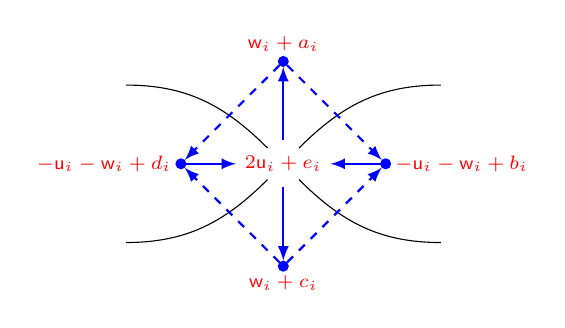
\begin{tikzpicture}
\begin{scope}[>=latex,xshift=0pt]
\draw [-] (0,2) to [out = 0, in = 135] (1.8,1.2);
\draw [-] (0,0) to [out = 0, in = -135] (1.8,0.8);
\draw [-] (2.2,0.8) to [out = -45, in = 180] (4,0);
\draw [-] (2.2,1.2) to [out = 45, in = 180] (4,2);
%
{\color{blue}
\fill (0.7,1) circle(2pt) coordinate(A) node[left]{\color{red} \scriptsize{$-\uu_i-\ww_i+d_i$}};
\fill (3.3,1) circle(2pt) coordinate(B) node[right]{\color{red} \scriptsize{$-\uu_i-\ww_i+b_i$}};
\fill (2,2.3) circle(2pt) coordinate(C) node[above]{\color{red} \scriptsize{$\ww_i+a_i$}};
\fill (2,-0.3) circle(2pt) coordinate(D) node[below]{\color{red} \scriptsize{$\ww_i+c_i$}};
\draw (2,1) node {\color{red} \scriptsize{$2\uu_i+e_i$}};
\draw[->,shorten >=2pt] (2,1.3) -- (C) [thick];
\draw[->,shorten >=2pt] (2,0.7) -- (D) [thick];
\draw[->] (A) -- (1.4,1) [thick];
\draw[->] (B) -- (2.6,1) [thick];
\qdarrow{C}{A}
\qdarrow{C}{B}
\qdarrow{D}{A}
\qdarrow{D}{B}
}
\end{scope}
\end{tikzpicture}
\caption{Graphical rule to parametrize the $Y$-variables in terms of
 $q$-Weyl algebra generators in the vicinity of the crossing $i$
 (center) of the wiring diagram (black). A $Y$-variable situated at
 a vertex (blue circle) of the symmetric butterfly quiver acquires
 factors $\e^{a_i+ \ww_i}$, $\e^{b_i-\uu_i-\ww_i}$, $\e^{c_i+\ww_i}$,
 $\e^{d_i-\uu_i-\ww_i}$ from the neighboring crossing $i$ of the wiring
 diagram if the vertex is located at the north, east, south, west of
 $i$, respectively. A $Y$-variable on the vertex $i$ is
 $\e^{e_i+2\uu_i}$. The ordering of these factors from different $i$'s
 (if any) is inconsequential due to the commutativity of the
 associated canonical variables. }\label{fig:para}
\end{figure}


The claim is that the relation
$Y_r Y_s = q^{2b_{rs}}Y_sY_r$ \eqref{yyq} is satisfied under this parametrization.
%
To state it formally, let $\mathcal{W}_n$ be the direct product of the
$q$-Weyl algebras generated by~$\e^{\pm \uu_i}$,~$\e^{\pm \ww_i}$ for
$i=1, \dots, n$. Let further $\mathcal{A}_n$ be the non-commuting
fractional field of $\mathcal{W}_n$. Then for $B$ corresponding to
the left diagram in Figure \ref{fig:R123}, we have a morphism
$\phi_\mathrm{SB}\colon \mathcal{Y}(B) \rightarrow \mathcal{A}_3$
defined by
\begin{align}
\phi_\mathrm{SB}\colon\
\begin{cases}
Y_1 \mapsto \e^{c_1+c_3+\ww_1+\ww_3},
& Y_6 \mapsto \e^{b_1-\uu_1-\ww_1},
\\
Y_2 \mapsto \e^{d_3-\uu_3-\ww_3},
& Y_7 \mapsto \e^{d_2+a_3-\uu_2-\ww_2+\ww_3},
\\
Y_3 \mapsto \e^{e_3+2\uu_3},
& Y_8 \mapsto \e^{e_2+2\uu_2},
\\
Y_4 \mapsto \e^{d_1+c_2+b_3-\uu_1-\ww_1+\ww_2-\uu_3-\ww_3},
& Y_9 \mapsto \e^{a_1+b_2+\ww_1-\uu_2-\ww_2},
\\
Y_5 \mapsto \e^{e_1+2\uu_1},
& Y_{10} \mapsto \e^{a_2+\ww_2},
\end{cases}
\label{Yw}
\end{align}
where SB signifies ``symmetric butterfly''. Similarly, for the right
diagram of Figure \ref{fig:R123}, we have a morphism
$\phi'_\mathrm{SB}\colon \mathcal{Y}\bigl(B'\bigr) \rightarrow \mathcal{A}_3$ as
\begin{align}
\phi'_\mathrm{SB}\colon\
\begin{cases}
Y'_1 \mapsto \e^{c_2+\ww_2},
& Y'_6 \mapsto \e^{b_2+c_3-\uu_2-\ww_2+\ww_3},
\\
Y'_2 \mapsto \e^{c_1+d_2+\ww_1-\uu_2-\ww_2},
& Y'_7 \mapsto \e^{d_1-\uu_1-\ww_1},
\\
Y'_3 \mapsto \e^{e_3+2\uu_3},
& Y'_8 \mapsto \e^{e_2+2\uu_2},
\\
Y'_4 \mapsto \e^{b_1+a_2+d_3-\uu_1-\ww_1+\ww_2-\uu_3-\ww_3},
& Y'_9 \mapsto \e^{b_3-\uu_3-\ww_3},
\\
Y'_5 \mapsto \e^{e_1+2\uu_1},
& Y'_{10} \mapsto \e^{a_1+a_3+\ww_1+\ww_3}.
\end{cases}
\label{Ypw}
\end{align}

\setcounter{Theorem}{1}\setcounter{equation}{6}
% Original source lines 2249--2512
\subsection[Extracting R\_123 from R\_123]{Extracting $\boldsymbol{R_{123}}$ from $\boldsymbol{\widehat{R}_{123}}$}

Let us illustrate the action of the monomial part
$\tau_{\varepsilon_1, \varepsilon_2, \varepsilon_3, \varepsilon_4}$
 \eqref{taue} of $\widehat{R}_{123}$ on the canonical variables for the case
 $(\varepsilon_1, \varepsilon_2, \varepsilon_3, \varepsilon_4) = (-,-,+,+)$.
 From Example \ref{ex:1} and \eqref{Yw}--\eqref{Ypw}, we find that
$\tau_{--++}$ is translated into a transformation $\tau^{\uu\ww}_{--++}$
of the canonical variables\footnote{$\tau^{\uu\ww}_{--++}$ is naturally regarded also as
a transformation in $\mathcal{W}_3$ via exponentials.} as
\begin{align}
\tau^{\uu\ww}_{--++}\colon\
\begin{cases}
\uu_1 \mapsto \uu_1+\uu_2-\uu_3+\lambda_0,
&
\ww_1 \mapsto \ww_1+ \lambda_1,
\\
\uu_2 \mapsto \uu_3-\lambda_0,
&
\ww_2 \mapsto \ww_1+\ww_3+\lambda_3,
\\
\uu_3 \mapsto \uu_2+\lambda_0,
&
\ww_3 \mapsto -\ww_1+\ww_2+\lambda_2,
\end{cases}
\label{uwL1}
\end{align}
where $\lambda_r=\lambda_r(\mathscr{P}_1,\mathscr{P}_2,\mathscr{P}_3)$
for $r=0, 1, 2, 3$ is defined, under the condition \eqref{ae0},
by
\begin{gather}
\lambda_0 = \frac{e_2-e_3}{2},\qquad
\lambda_1 = a_2-a_3+b_2-b_3 + \lambda_0,\qquad
\lambda_2 = -a_1-b_2+b_3-\lambda_0,\nonumber\\
\lambda_3 = c_1-c_2+c_3.\label{lad}
\end{gather}

In order to realize \eqref{uwL1} as an adjoint action, we introduce
the group $N_n$ generated by
\begin{gather*}
\e^{\pm \tfrac{1}{\hbar}\uu_i\ww_j}\quad (i \neq j),\qquad
\e^{ \tfrac{a}{\hbar}\uu_i}, \qquad \e^{ \tfrac{a}{\hbar}\ww_i}  \quad (a \in \C) ,\qquad b \in \C^\times
\end{gather*}
with $i, j\in \{1,\dotsc, n\}$. The multiplication is defined by
the (generalized) Baker--Campbell--Hausdorff (BCH) formula and
\eqref{uwh}, which is well defined due to the grading by $\hbar^{-1}$.
Let $\mathfrak{S}_n$ be the symmetric group generated by the
transpositions $\rho_{ij}$ ($i, j \in \{1,\dotsc, n\}$). It acts on
$N_n$ via the adjoint action, inducing permutations of the indices of
the canonical variables. Thus one can form the semi-direct product
$N_n \rtimes \mathfrak{S}_n$, and let it act on $\mathcal{W}_n$ by the
adjoint action.

Now the monomial part $\tau^{\uu\ww}_{--++}$
is described as the adjoint action as follows:
\begin{align}
&\tau^{\uu\ww}_{--++} = \mathrm{Ad}(P_{--++}),
\label{Pbch0}\\
&P_{--++}=
\e^{\tfrac{1}{\hbar}(\uu_3-\uu_2)\ww_1}
\e^{\tfrac{\lambda_0}{\hbar}(-\ww_1-\ww_2+\ww_3)}
\e^{\tfrac{1}{\hbar}(\lambda_1\uu_1+\lambda_2\uu_2+\lambda_3\uu_3)}\rho_{23}
\in N_3 \rtimes \mathfrak{S}_3,
\label{Pbch1}
\end{align}
where $\rho_{23}$ acts trivially on the parameters $\lambda_r$.
%
Extending the indices and suppressing the sign choice of $--++$ in \eqref{Pbch0} and \eqref{Pbch1}, we introduce
\begin{align}
\tau^{\uu\ww}_{ijk} &= \mathrm{Ad}(P_{ijk}),
\label{tijk}\\
P_{ijk} &=
\e^{\tfrac{1}{\hbar}(\uu_k-\uu_j)\ww_i}
\e^{\tfrac{\lambda_0}{\hbar}(-\ww_i-\ww_j+\ww_k)}
\e^{\tfrac{1}{\hbar}(\lambda_1\uu_i+\lambda_2\uu_j+\lambda_3\uu_k)}\rho_{jk}
\in N_6 \rtimes \mathfrak{S}_6,
\label{pijk}
\end{align}
where $\lambda_r=\lambda_r(\mathscr{P}_i, \mathscr{P}_j, \mathscr{P}_k)$ is given by
\eqref{lad} by replacing the parameters as
$(\mathscr{P}_1 ,\mathscr{P}_2 ,\mathscr{P}_3) \rightarrow
(\mathscr{P}_i ,\mathscr{P}_j ,\mathscr{P}_k)$.
%
By a straightforward calculation using the BCH formula, one can prove the following.
\begin{Lemma}\label{le:tep}
$P_{ijk}$ satisfies the tetrahedron equation in $N_6 \rtimes \mathfrak{S}_6$ by itself
\begin{align}\label{pte}
P_{124}P_{135}P_{236}P_{456} =
P_{456}P_{236}P_{135}P_{124}.
\end{align}
\end{Lemma}
The fact that $P_{ijk}$ acts on the canonical variables rather than $Y$-variables
has led to the tetrahedron equation {\em without} a twist by permutations.

Define $R_{123}= R(\mathscr{P}_1,\mathscr{P}_2,\mathscr{P}_3)_{123}$ by
\begin{align}
R_{123}
={}&
\Psi_q\bigl(\e^{-d_1-c_2-b_3+\uu_1+\uu_3+\ww_1-\ww_2+\ww_3}\bigr)^{-1}
\Psi_q\bigl(\e^{-d_1-c_2-b_3-e_3+\uu_1-\uu_3+\ww_1-\ww_2+\ww_3}\bigr)^{-1}
\nonumber \\
& \times
\Psi_q\bigl(\e^{d_1+e_1+c_2+b_3+\uu_1-\uu_3-\ww_1+\ww_2-\ww_3}\bigr)\nonumber \\
& \times
\Psi_q\bigl(\e^{d_1+e_1+c_2+e_2+b_3+\uu_1+2\uu_2-\uu_3-\ww_1+\ww_2-\ww_3}\bigr)P_{123}
\label{RL0}
\\
={}&
\Psi_q\bigl(\e^{-d_1-c_2-b_3+\uu_1+\uu_3+\ww_1-\ww_2+\ww_3}\bigr)^{-1}
\Psi_q\bigl(\e^{-d_1-c_2-b_3-e_3+\uu_1-\uu_3+\ww_1-\ww_2+\ww_3}\bigr)^{-1}
\nonumber\\
& \times P_{123}
\Psi_q\bigl(\e^{-b_1-a_2-d_3-e_3+\uu_1-\uu_3+\ww_1-\ww_2+\ww_3}\bigr)\nonumber \\
& \times
\Psi_q\bigl(\e^{-b_1-a_2-d_3+\uu_1+\uu_3+\ww_1-\ww_2+\ww_3}\bigr).
\label{RL1}
\end{align}
Let $\widehat{R}^{\uu\ww}_{123}$ be the cluster transformation $\widehat{R}_{123}$ \eqref{dode}
viewed as the one for the canonical variables~${\{\uu_i, \ww_i\}_{i=1,2,3}}$.
%
Then from \eqref{Yw}, \eqref{Ypw} and \eqref{Pbch0}, we have
\begin{align}\label{knm}
\widehat{R}^{\uu\ww}_{123} &= \mathrm{Ad}\bigl(R(\mathscr{P}_1,\mathscr{P}_2,\mathscr{P}_3)_{123}\bigr).
\end{align}
Note that the right-hand side is invariant under $R \rightarrow cR$ for any scalar $c$.
A proper normalization of $R$ based on a symmetry consideration will be proposed
in Section \ref{ss:symR}.

Formally the results \eqref{uwL1} and \eqref{knm} may be stated as the commutativity of the diagrams
\begin{align*}%\label{Rcom}
\begin{CD}
\mathcal{Y}\bigl(B'\bigr) @> {\tau_{--++}}>> \mathcal{Y}(B) \\
@V{\phi'_\mathrm{SB}}VV @VV{\phi_\mathrm{SB}}V \\
\mathcal{A}_3 @>{\tau^{\uu\ww}_{--++}}>> \mathcal{A}_3,
\end{CD}
\qquad\qquad
\begin{CD}
\mathcal{Y}\bigl(B'\bigr) @> {\widehat{R}_{123}}>> \mathcal{Y}(B) \\
@V{\phi'_\mathrm{SB}}VV @VV{\phi_\mathrm{SB}}V \\
\mathcal{A}_3 @>{\widehat{R}^{\uu\ww}_{123}}>> \mathcal{A}_3.
\end{CD}
\end{align*}

Extending \eqref{RL0} and \eqref{RL1}, we introduce
$R_{ijk}=R(\mathscr{P}_i ,\mathscr{P}_j ,\mathscr{P}_k)_{ijk}$
by
\begin{align}
R_{ijk}
={}&
\Psi_q\bigl(\e^{-d_i-c_j-b_k+\uu_i+\uu_k+\ww_i-\ww_j+\ww_k}\bigr)^{-1}
\Psi_q\bigl(\e^{-d_i-c_j-b_k-e_k+\uu_i-\uu_k+\ww_i-\ww_j+\ww_k}\bigr)^{-1}
\nonumber \\
& \times
\Psi_q\bigl(\e^{d_i+e_i+c_j+b_k+\uu_i-\uu_k-\ww_i+\ww_j-\ww_k}\bigr)\nonumber \\
& \times
\Psi_q\bigl(\e^{d_i+e_i+c_j+e_j+b_k+\uu_i+2\uu_j-\uu_k-\ww_i+\ww_j-\ww_k}\bigr)P_{ijk}
\label{rijk0}\\
={}&
\Psi_q\bigl(\e^{-d_i-c_j-b_k+\uu_i+\uu_k+\ww_i-\ww_j+\ww_k}\bigr)^{-1}
\Psi_q\bigl(\e^{-d_i-c_j-b_k-e_k+\uu_i-\uu_k+\ww_i-\ww_j+\ww_k}\bigr)^{-1}
\nonumber\\
& \times P_{ijk}
\Psi_q\bigl(\e^{-b_i-a_j-d_k-e_k+\uu_i-\uu_k+\ww_i-\ww_j+\ww_k}\bigr)
\Psi_q\bigl(\e^{-b_i-a_j-d_k+\uu_i+\uu_k+\ww_i-\ww_j+\ww_k}\bigr),
\label{rijk}
\end{align}
where $P_{ijk}$ is given by \eqref{pijk}.
Now we state the main result of the paper.

\begin{Theorem}\label{th:main}
$R(\mathscr{P}_i, \mathscr{P}_j, \mathscr{P}_k)_{ijk} $ satisfies the tetrahedron equation
\begin{gather}
 R(\mathscr{P}_1, \mathscr{P}_2, \mathscr{P}_4)_{124}
R(\mathscr{P}_1, \mathscr{P}_3, \mathscr{P}_5)_{135}
R(\mathscr{P}_2, \mathscr{P}_3, \mathscr{P}_6)_{236}
R(\mathscr{P}_4, \mathscr{P}_5, \mathscr{P}_6)_{456}\nonumber
\\
\qquad= R(\mathscr{P}_4, \mathscr{P}_5, \mathscr{P}_6)_{456}
R(\mathscr{P}_2, \mathscr{P}_3, \mathscr{P}_6)_{236}
R(\mathscr{P}_1, \mathscr{P}_3, \mathscr{P}_5)_{135}
R(\mathscr{P}_1, \mathscr{P}_2, \mathscr{P}_4)_{124}.\label{tela}
\end{gather}
\end{Theorem}
\begin{proof}
 Consider the dilogarithm identity \eqref{pseq} with
 $(\varepsilon_1,\varepsilon_2,\varepsilon_3,\varepsilon_4) =(-, -,
 +, +)$ in terms of canonical variables\footnote{The signs
 $\varepsilon_1$, $\varepsilon_2$, $\varepsilon_3$, $\varepsilon_4$
 are actually $-$, $-$, $+$, $+$, but for clarity, they are left as
 they are.}
\begin{align}\label{zt16}
\Psi_q\bigl(\tilde{Z}_1\bigr)^{\varepsilon_1}\dotsm \Psi_q\bigl({\tilde Z}_{16}\bigr)^{\varepsilon_4}
=
\Psi_q\bigl(\tilde{Z'}_1\bigr)^{\varepsilon_1}\dotsm \Psi_q\bigl(\tilde{Z'}_{16}\bigr)^{\varepsilon_4}.
\end{align}
Here $\tilde{Z}_i = \tilde{\phi}_\mathrm{SB}(Z_i)$ and
$\tilde{Z'}_i =\tilde{\phi}'_\mathrm{SB}(Z'_i)$ with $Z_i$ and $Z'_i$
given in \eqref{zdL} and \eqref{zdR}. The morphisms~$\tilde{\phi}_\mathrm{SB}$ and $\tilde{\phi}'_\mathrm{SB}$ are natural
generalizations of \eqref{Yw} and \eqref{Ypw}. They send the
$Y$-variables to $\mathcal{W}_6$ according to the rule in Figure
\ref{fig:para} applied to the bottom right diagram in Figure
\ref{fig:bTE}.\footnote{The map $\phi_\mathrm{SB}$ does not spoil the
 well-definedness of the expansion like \eqref{c16} with respect to
 $\e^{\uu_i}$ and $\e^{\ww_i}$ since it preserves the rank of the quantum
 torus generated by $Y_i$ ($i=3, 6 , 7 , 8 , 11 , 12 , 13 ,
 14 , 15$).}
%
Multiplication of \eqref{pte} to \eqref{zt16} from the right leads to
\begin{gather}
\Psi_q\bigl(\tilde{Z}_1\bigr)^{\varepsilon_1}\dotsm \Psi_q\bigl({\tilde Z}_{16}\bigr)^{\varepsilon_4}
P_{124}P_{135}P_{236}P_{456}\nonumber\\
\qquad=
\Psi_q\bigl(\tilde{Z'}_1\bigr)^{\varepsilon_1}\dotsm \Psi_q\bigl(\tilde{Z'}_{16}\bigr)^{\varepsilon_4}
P_{456}P_{236}P_{135}P_{124}.\label{zp16}
\end{gather}
Let us consider the left-hand side.
It is obviously equal to
\begin{gather}
\Psi_q\bigl(\tilde{Z}_1\bigr)^{\varepsilon_1}\dotsm \Psi_q\bigl({\tilde Z}_{4}\bigr)^{\varepsilon_4}
P_{124}
P^{-1}_{124}
\Psi_q\bigl(\tilde{Z}_5\bigr)^{\varepsilon_1}\dotsm \Psi_q\bigl({\tilde Z}_{8}\bigr)^{\varepsilon_4}
P_{124} \cdot P_{135}\nonumber
\\
\qquad \times
P^{-1}_{135} P^{-1}_{124}
\Psi_q\bigl(\tilde{Z}_9\bigr)^{\varepsilon_1}\dotsm \Psi_q\bigl({\tilde Z}_{12}\bigr)^{\varepsilon_4}
P_{124} P_{135} \cdot P_{236}\nonumber
\\
\qquad \times
P^{-1}_{236} P^{-1}_{135} P^{-1}_{124}
\Psi_q\bigl(\tilde{Z}_{13}\bigr)^{\varepsilon_1}\dotsm \Psi_q\bigl({\tilde Z}_{16}\bigr)^{\varepsilon_4}
P_{124} P_{135} P_{236} \cdot P_{456}.\label{tochu1}
\end{gather}
On the other hand from \eqref{tijk} and the image of $\eqref{zu}$ by $\tilde{\phi}_\mathrm{SB}$, we know
\begin{align*}
{\tilde U}_i = \begin{cases}
\tilde{Z}_i, & i=1,\dotsc, 4,
\\
P_{124}^{-1} \tilde{Z}_i P_{124}, & i=5,\dotsc, 8,
\\
P_{135}^{-1}P_{124}^{-1} \tilde{Z}_i P_{124}P_{135}, & i=9,\dotsc, 12,
\\
P_{236}^{-1}P_{135}^{-1}P_{124}^{-1} \tilde{Z}_i
P_{124}P_{135} P_{236}, & i=13,\dotsc, 16,
\end{cases}
\end{align*}
where $\tilde{U}_i = \tilde{\phi}_\mathrm{SB}(U_i)$.
Thus \eqref{tochu1} is cast into the form
\begin{gather*}
\Psi_q\bigl(\tilde{U}_1\bigr)^{\varepsilon_1}\cdots \Psi_q\bigl({\tilde U}_{4}\bigr)^{\varepsilon_4}
P_{124}
\Psi_q\bigl(\tilde{U}_5\bigr)^{\varepsilon_1}\cdots \Psi_q\bigl({\tilde U}_{8}\bigr)^{\varepsilon_4}
P_{135}
\\
\qquad\times
\Psi_q\bigl(\tilde{U}_9\bigr)^{\varepsilon_1}\cdots \Psi_q\bigl({\tilde U}_{12}\bigr)^{\varepsilon_4}
P_{236}
\Psi_q\bigl(\tilde{U}_{13}\bigr)^{\varepsilon_1}\cdots \Psi_q\bigl({\tilde U}_{16}\bigr)^{\varepsilon_4}
P_{456}.
\end{gather*}
This is identified with the left-hand side of \eqref{tela} for \eqref{rijk0}.
The right-hand side of \eqref{tela} is similarly derived from that in \eqref{zp16}.
\end{proof}

\setcounter{section}{0}
% Original source lines 4702--4766
\appendix

\section[Supplement to Section 3.4]{Supplement to Section \ref{ss:ms}}\label{ap:sup}

The two sides of the inhomogeneous twisted tetrahedron equation \eqref{ihte} yield the
following monomial transformation:
\begin{gather}
Y^{(22)}_1 \mapsto Y_1, \qquad
Y^{(22)}_2 \mapsto Y_2, \qquad
Y^{(22)}_3 \mapsto qY^{-1}_{7}Y^{-1}_{12}Y^{-1}_{13}Y^{-1}_{14},\qquad
Y^{(22)}_4 \mapsto Y_4,\nonumber
\\
Y^{(22)}_5 \mapsto q^{-1}Y_5Y_6, \qquad
Y^{(22)}_6 \mapsto q Y_{13}Y_{14}, \qquad
Y^{(22)}_7 \mapsto Y^{-1}_{13},\qquad
Y^{(22)}_{8} \mapsto q^{-1}Y_{12}Y_{13},\nonumber\\
Y^{(22)}_{9} \mapsto qY_{8}Y_{9},
\qquad
Y^{(22)}_{10} \mapsto q^{-1}Y_{10}Y_{11}, \qquad
Y^{(22)}_{11} \mapsto Y_3Y_6Y_7Y_{11}Y_{12},\nonumber\\
Y^{(22)}_{12} \mapsto q^{-3}Y^{-1}_{3}Y^{-1}_{6}Y^{-1}_{7}Y^{-1}_{8}Y^{-1}_{14}Y^{-1}_{15},
\qquad
Y^{(22)}_ {13} \mapsto q^{-1}Y_3Y_6Y_7Y_8,\nonumber\\
Y^{(22)}_{14} \mapsto q^{-1}Y^{-1}_{3}Y^{-1}_{6}Y^{-1}_{7}Y^{-1}_{8}Y^{-1}_{11}Y^{-1}_{12},\qquad
Y^{(22)}_ {15} \mapsto q^{-4}Y_3Y_7Y_8Y_{14}Y_{15},\nonumber\\
Y^{(22)}_{16} \mapsto qY_{15}Y_{16},\qquad
Y^{(22)}_{17} \mapsto q^{2}Y_7Y_{12}Y_{13}Y_{14}Y_{17}.\label{y22}
\end{gather}

Let us describe the monomial parts $\tau_{-+++}$ and $\tau_{---+}$ in \eqref{taue} mentioned
in Proposition \ref{pr:mono}
\begin{gather*}
\tau_{-+++}\colon\
\begin{cases}
Y'_1 \mapsto Y_1,\qquad
Y'_2 \mapsto Y_2Y_3Y_4, \qquad
Y'_3 \mapsto q^2Y_3Y_4Y_8, \\ \qquad
Y'_4 \mapsto q^2Y^{-1}_3Y^{-2}_4Y^{-1}_5Y^{-1}_8,
\\
Y'_5 \mapsto Y_4Y_5Y_8, \qquad
Y'_6 \mapsto Y_4 Y_5 Y_6,\qquad
Y'_7 \mapsto Y_7,\qquad
Y'_8 \mapsto Y^{-1}_4,
\\
Y'_9 \mapsto Y_9, \qquad
Y'_{10} \mapsto Y_{10},
\end{cases}
\\
 \tau_{---+}\colon\
\begin{cases}
Y'_1 \mapsto Y_1,\qquad
Y'_2 \mapsto Y_2, \qquad
Y'_3 \mapsto q^{-2}Y^{-1}_4Y^{-1}_5Y_8, \qquad
Y'_4 \mapsto Y^{-1}_8, \qquad
\\
Y'_5 \mapsto Y^{-1}_3Y^{-1}_4Y_8, \qquad
Y'_6 \mapsto Y_6,\qquad
Y'_7 \mapsto Y_3Y_4Y_7,\qquad
Y'_8 \mapsto Y_3Y_4Y_5,
\\
Y'_9 \mapsto q^{-2} Y_4Y_5Y_9, \qquad
Y'_{10} \mapsto Y_{10}.
\end{cases}
\end{gather*}
Note that the image is not necessarily sign coherent.
\section*{Editable literal labels for original Figure5 (transcription)}
\noindent\textbf{Editorial locator convention:} The unchanged original \texttt{tetra-butterfly.pdf} remains the geometric diagram. Its ten panels are L0--L4 in the left column and R0--R4 in the right column, each top to bottom. Within each panel, the following rows are literal labels grouped by horizontal node tier, from the top blue apex to the bottom blue apex, left to right within a tier. Red rows group the printed crossing labels by their horizontal tier, top to bottom and left to right. These are location-bound text transcriptions, not a recomputed exchange matrix or inferred arrow list. Every blue/red mathematical label and interpanel jump label is editable below; the original coloured geometry is unchanged.\par
\medskip\noindent\textbf{Panel L0:} $B^{(22)}=B^{(22)\prime}$.\par
\noindent Blue vertex-label tiers: $(1)\ ;\ (2,15,12,13,14,11,4)\ ;\ (5,8,7,6,9)\ ;\ (10,3,16)\ ;\ (17)$.\par
\noindent Red crossing-label tiers: $(1,4,6)\ ;\ (2,5)\ ;\ (3)$.\par
\medskip\noindent\textbf{Panel R0:} $B^{(21)\prime}$.\par
\noindent Blue vertex-label tiers: $(1)\ ;\ (2,15,12,13,7,11,4)\ ;\ (5,8,14,6,9)\ ;\ (10,3,16)\ ;\ (17)$.\par
\noindent Red crossing-label tiers: $(1,4,6)\ ;\ (2,5)\ ;\ (3)$.\par
\medskip\noindent\textbf{Panel L1:} $B^{(21)}$.\par
\noindent Blue vertex-label tiers: $(1)\ ;\ (2,15,7,13,14,11,4)\ ;\ (5,8,12,6,9)\ ;\ (10,3,16)\ ;\ (17)$.\par
\noindent Red crossing-label tiers: $(1,4,6)\ ;\ (2,5)\ ;\ (3)$.\par
\medskip\noindent\textbf{Panel R1:} $B^{(16)\prime}$.\par
\noindent Blue vertex-label tiers: $(1)\ ;\ (2,8,7,11,4)\ ;\ (5,13,12,15,14,6,9)\ ;\ (10,3,16)\ ;\ (17)$.\par
\noindent Red crossing-label tiers: $(2,6)\ ;\ (4,1,5)\ ;\ (3)$.\par
\medskip\noindent\textbf{Panel L2:} $B^{(16)}$.\par
\noindent Blue vertex-label tiers: $(1)\ ;\ (2,15,7,6,4)\ ;\ (5,8,12,11,14,13,9)\ ;\ (10,3,16)\ ;\ (17)$.\par
\noindent Red crossing-label tiers: $(1,5)\ ;\ (2,6,4)\ ;\ (3)$.\par
\medskip\noindent\textbf{Panel R2:} $B^{(11)\prime}$.\par
\noindent Blue vertex-label tiers: $(1)\ ;\ (2,8,7,11,4)\ ;\ (5,13,12,3,9)\ ;\ (10,6,14,15,16)\ ;\ (17)$.\par
\noindent Red crossing-label tiers: $(2,6)\ ;\ (4,3)\ ;\ (5,1)$.\par
\medskip\noindent\textbf{Panel L3:} $B^{(11)}$.\par
\noindent Blue vertex-label tiers: $(1)\ ;\ (2,15,7,6,4)\ ;\ (5,3,14,13,9)\ ;\ (10,11,12,8,16)\ ;\ (17)$.\par
\noindent Red crossing-label tiers: $(1,5)\ ;\ (3,4)\ ;\ (6,2)$.\par
\medskip\noindent\textbf{Panel R3:} $B^{(6)\prime}$.\par
\noindent Blue vertex-label tiers: $(1)\ ;\ (2,3,4)\ ;\ (5,13,12,11,7,8,9)\ ;\ (10,6,14,15,16)\ ;\ (17)$.\par
\noindent Red crossing-label tiers: $(3)\ ;\ (4,6,2)\ ;\ (5,1)$.\par
\medskip\noindent\textbf{Panel L4:} $B^{(6)}$.\par
\noindent Blue vertex-label tiers: $(1)\ ;\ (2,3,4)\ ;\ (5,6,7,15,14,13,9)\ ;\ (10,11,12,8,16)\ ;\ (17)$.\par
\noindent Red crossing-label tiers: $(3)\ ;\ (5,1,4)\ ;\ (6,2)$.\par
\medskip\noindent\textbf{Panel R4:} $B^{(1)}=B^{(1)\prime}$.\par
\noindent Blue vertex-label tiers: $(1)\ ;\ (2,3,4)\ ;\ (5,6,7,8,9)\ ;\ (10,11,12,13,14,15,16)\ ;\ (17)$.\par
\noindent Red crossing-label tiers: $(3)\ ;\ (5,2)\ ;\ (6,4,1)$.\par
\medskip\noindent\textbf{Literal interpanel arrow labels and visibly printed directions:}\par
\begin{itemize}\itemsep=0pt
\item L0 to R0: $\sigma_{7,14}$, right.
\item L0 to L1: $\sigma_{7,12}$, down.
\item L1 to L2: $\widehat{R}_{456}$, down.
\item L2 to L3: $\widehat{R}_{236}$, down.
\item L3 to L4: $\widehat{R}_{135}$, down.
\item L4 to R4: $\widehat{R}_{124}$, right.
\item R0 to R1: $\widehat{R}_{124}$, down.
\item R1 to R2: $\widehat{R}_{135}$, down.
\item R2 to R3: $\widehat{R}_{236}$, down.
\item R3 to R4: $\widehat{R}_{456}$, down.
\end{itemize}

\begin{thebibliography}{99}
\bibitem[5]{FG06}
Fock V.V., Goncharov A.B., Cluster {$\mathcal{X}$}-varieties, amalgamation, and
 {P}oisson--{L}ie groups, in Algebraic {G}eometry and {N}umber {T}heory,
 \textit{Progr. Math.}, Vol. 253, \href{https://doi.org/10.1007/978-0-8176-4532-8_2}{Birkh\"auser Boston}, Boston, MA, 2006,
 27--68, \href{https://arxiv.org/abs/math.RT/0508408}{arXiv:math.RT/0508408}.

\bibitem[6]{FG09}
Fock V.V., Goncharov A.B., Cluster ensembles, quantization and the dilogarithm,
 \href{https://doi.org/10.24033/asens.2112}{\textit{Ann. Sci. \'Ec. Norm. Sup\'er.}} \textbf{42} (2009), 865--930,
 \href{https://arxiv.org/abs/math.AG/0311245}{arXiv:math.AG/0311245}.

\bibitem[7]{FG09b}
Fock V.V., Goncharov A.B., The quantum dilogarithm and representations of
 quantum cluster varieties, \href{https://doi.org/10.1007/s00222-008-0149-3}{\textit{Invent. Math.}} \textbf{175} (2009),
 223--286, \href{https://arxiv.org/abs/math.QA/0702397}{arXiv:math.QA/0702397}.

\bibitem[8]{FZ07}
Fomin S., Zelevinsky A., Cluster algebras.~{IV}. {C}oefficients,
 \href{https://doi.org/10.1112/S0010437X06002521}{\textit{Compos. Math.}} \textbf{143} (2007), 112--164,
 \href{https://arxiv.org/abs/math.RA/0602259}{arXiv:math.RA/0602259}.

\bibitem[10]{GHKK14}
Gross M., Hacking P., Keel S., Kontsevich M., Canonical bases for cluster
 algebras, \href{https://doi.org/10.1090/jams/890}{\textit{J.~Amer. Math. Soc.}} \textbf{31} (2018), 497--608,
 \href{https://arxiv.org/abs/1411.1394}{arXiv:1411.1394}.

\bibitem[15]{KN11}
Kashaev R.M., Nakanishi T., Classical and quantum dilogarithm identities,
 \href{https://doi.org/10.3842/SIGMA.2011.102}{\textit{SIGMA}} \textbf{7} (2011), 102, 29~pages, \href{https://arxiv.org/abs/1104.4630}{arXiv:1104.4630}.

\bibitem[16]{Ke11}
Keller B., On cluster theory and quantum dilogarithm identities, in
 Representations of {A}lgebras and {R}elated {T}opics, \textit{EMS Ser. Congr. Rep.},
 \href{https://doi.org/10.4171/101-1/3}{European Mathematical Society}, Z\"urich, 2011, 85--116, \href{https://arxiv.org/abs/1102.4148}{arXiv:1102.4148}.

\bibitem[19]{N11}
Nakanishi T., Periodicities in cluster algebras and dilogarithm identities, in
 Representations of {A}lgebras and {R}elated {T}opics, \textit{EMS Ser. Congr. Rep.},
 \href{https://doi.org/10.4171/101-1/9}{European Mathematical Society}, Z\"urich, 2011, 407--443, \href{https://arxiv.org/abs/1006.0632}{arXiv:1006.0632}.

\bibitem[20]{N21}
Nakanishi T., Synchronicity phenomenon in cluster patterns, \href{https://doi.org/10.1112/jlms.12402}{\textit{J.~Lond.
 Math. Soc.}} \textbf{103} (2021), 1120--1152, \href{https://arxiv.org/abs1906.12036}{arXiv:1906.12036}.

\bibitem[23]{SY22}
Sun X., Yagi J., Cluster transformations, the tetrahedron equation and
 three-dimensional gauge theories, \href{https://doi.org/10.4310/atmp.2023.v27.n4.a2}{\textit{Adv. Theor. Math. Phys.}}
 \textbf{27} (2023), 1065--1106, \href{https://arxiv.org/abs/2211.10702}{arXiv:2211.10702}.

\end{thebibliography}
\end{document}
